
\documentclass{article}
\usepackage[a4paper, margin=1in]{geometry}
\usepackage[hidelinks]{hyperref}
\usepackage{xcolor}
\usepackage{graphicx}

% Set graphics path to images/ folder
\graphicspath{{../Image/}}

\title{\LARGE \textbf{Python for Data Science: A Comprehensive Guide to Analysis, Machine Learning, and Big Data}}
\author{Nikita Kanhu Das}
\date{\today}
\begin{document}

\maketitle
\tableofcontents
\newpage
\section{Introduction to Data Science with Python}

\subsection{What is Data Science?}
Data Science is a multidisciplinary domain of study that includes statistical analysis, machine learning, data visualization, and computer programming to infer useful insights from data. Data Science encompasses different processes such as data collection, cleaning, exploration, modeling, and interpretation. Data Science is used on a large scale in various domains like healthcare, finance, marketing, and artificial intelligence to inform data-driven decisions.
\newline
\newline
\textbf{Key Data Science Elements}:
\begin{itemize}
    \item \textbf{Data Collection}: Collecting raw data from varied sources.
    \item \textbf{Data Purification}: Cleansing and sanitizing data for analysis.
    \item \textbf{Exploratory Data Analysis (EDA)}: A preview of patterns, trends, and distributions of the data.
    \item \textbf{Machine Learning}: Developing predictive models using algorithms.
    \item \textbf{Data Visualization}: Turning data insights into graphs and charts.
    \item \textbf{Conclusion Formation \& Decision Making}: Creating conclusions from data insights to plan.
\end{itemize}
\subsection{Why Use Python for Data Science?}
Python has emerged as the top programming language for Data Science because it is easy, flexible, and encompasses a huge universe of libraries specific to data manipulation, analysis, and machine learning.
\newline
\newline
\textbf{Benefits of Python for Data Science}:

\begin{itemize}
    \item \textbf{Ease of Use}: Python's syntax is easy and readable, and hence it is ideal for beginners. 
    \item \textbf{Extensive Libraries}: Dense collection of libraries for data manipulation, visualization, and machine learning.
    \item \textbf{Strong Community Support}: Big open-source community with ongoing enhancements and support.
    \item \textbf{Integration Capabilities}: Smooth integration with databases, big data solutions, and cloud infrastructure.
    \item \textbf{Scalability}: Adaptable to small-scale tests and big-scale enterprise uses.
\end{itemize}

\subsection{Popular Python Libraries for Data Science}
Python provides numerous libraries that help Data Science activities such as data manipulation, data visualization, and machine learning.
\newline
\newline`
\textbf{Some Popular Python Libraries}:
\begin{itemize}
    \item \textbf{NumPy}: Employs large multi-dimensional matrices and arrays, together with mathematical operations.
    \item \textbf{Pandas}: Offers data structures such as DataFrames for processing structured data in an efficient way.
    \item \textbf{Matplotlib \& Seaborn}: Data animated, static, and interactive plotting libraries.
    \item \textbf{Scikit-learn}: Machine learning library for offering support for algorithms of classification, regression, and clustering.
    \item \textbf{TensorFlow \& PyTorch}: Libraries for building and training deep learning neural networks.
    \item \textbf{Statsmodels}: Statistical modeling and testing using hypothesis.
    \item \textbf{NLTK \& spaCy}: NLP activities such as tokenizing and sentiment analysis libraries.
    \item \textbf{SciPy}: Offers higher-level mathematical functions and signal processing.
    \item \textbf{Dask \& Vaex}: Big data processing libraries using Python.
\end{itemize}
Python remains one of the most shaping and popular programming languages, adapting itself with emerging technologies and uses.
\subsection{Example of Python Code}
Here’s a simple Python program that prints “Hello, World!”:

\begin{figure}[htbp]
\centerline{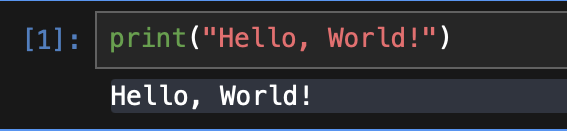
\includegraphics[width=10cm,height=2cm]{Example.png}}
\label{fig}
\end{figure}

\newpage
\section{Python Libraries for Data Science}
Data science is based on a set of robust Python libraries that support effective data manipulation, analysis, visualization, and machine learning. The next section gives an overview of some of the most important libraries used in data science and their applications.
\subsection{NumPy – Numerical Computing}

\begin{itemize}
    \item NumPy, or Numerical Python, is a core library for numerical computation in Python.
    \item It offers support for large multi-dimensional matrices and arrays, as well as a set of mathematical functions to perform operations on the arrays.
    \item  NumPy increases performance by using an optimized C-based implementation, which facilitates high-speed numerical computation.
    \item \textbf{Major Features}:
    \begin{itemize}
    \item Support for multi-dimensional arrays (ndarray).
    \item Mathematical and statistical functionalities.
    \item Linear algebra and Fourier transform functionality.
    \item Random number generation.
    \item Interoperability with other scientific libraries.
    \end{itemize}

\end{itemize}

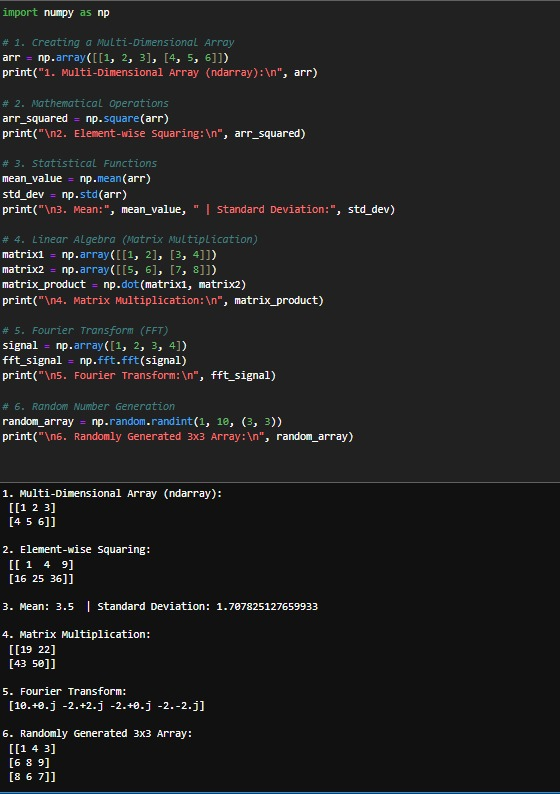
\includegraphics[width=14cm,height=15cm]{NumPy.jpeg}
\newpage
\subsection{Pandas – Data Manipulation}
\begin{itemize}
    \item Pandas is a high-performance library intended for data manipulation and analysis.
    \item It presents two primary data structures: Series (one-dimensional) and DataFrame (two-dimensional), which facilitate efficient data handling and processing.
    \item \textbf{Main Features}:
    \begin{itemize}
    \item DataFrame and Series for storing structured data.
    \item Data cleaning and data transformation.
    \item Missing data handling.
    \item Merging, grouping, and filtering data sets.
    \item Support for time series analysis.
    \end{itemize}
\end{itemize}
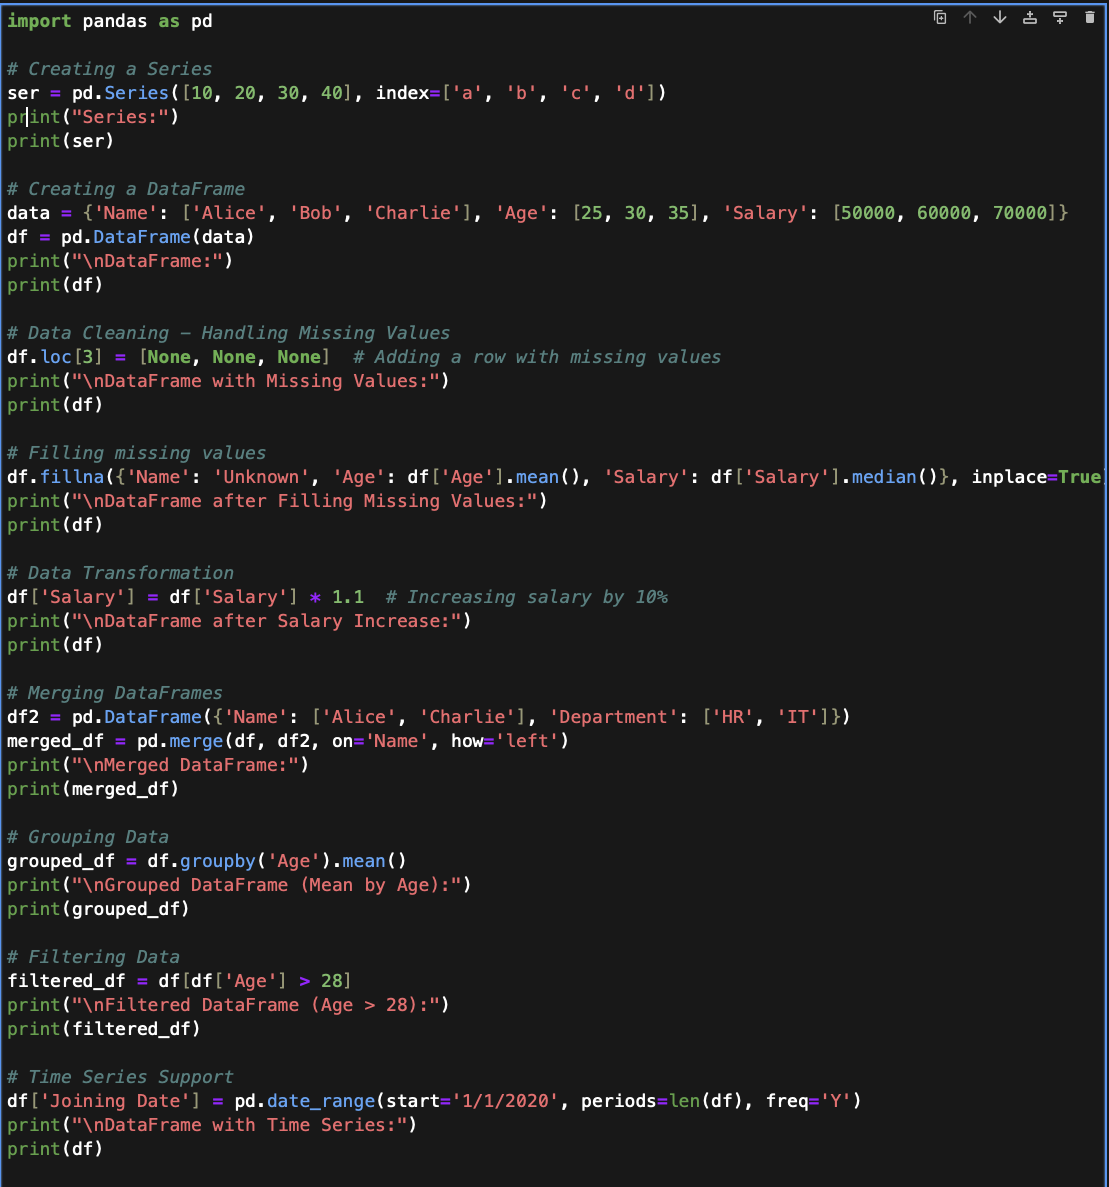
\includegraphics[width=14
cm,height=19cm]{Pandas.png}

\textbf{Output}:

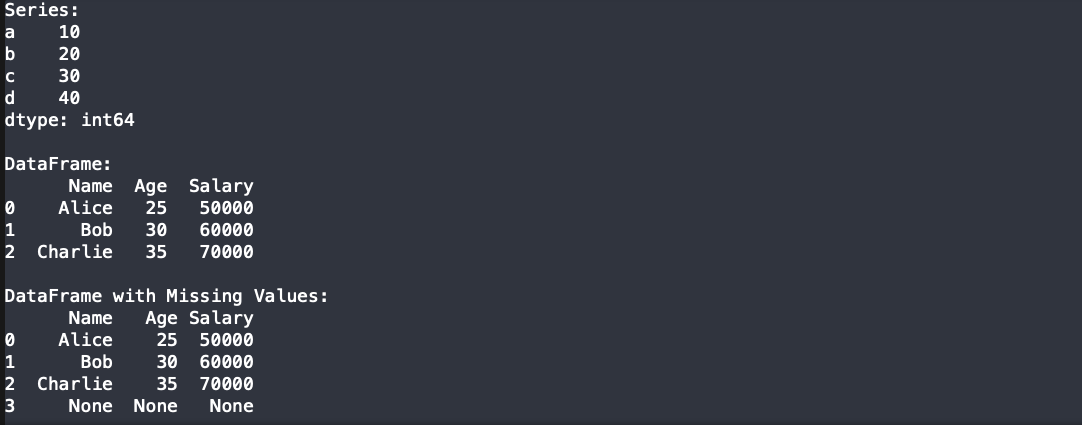
\includegraphics[width=14
cm,height=6cm]{Pandas_Output.png}
\subsection{Matplotlib \& Seaborn – Data Visualization}
\begin{itemize}
    \item Matplotlib is a robust library for static, animated, and interactive Python visualizations.
    \item Seaborn, which is based on Matplotlib, makes statistical data visualization easier with more aesthetics and functionalities.
\item \textbf{Key Features}:
    \begin{itemize}
    \item Plots with customizable appearances (line charts, bar graphs, histograms, scatter plots, etc.).
    \item State-based and object-oriented plotting interface.
    \item Thematic visualization and statistical plotting (Seaborn).
    \item Support for intricate multi-plot layouts.
    \end{itemize}
\end{itemize}
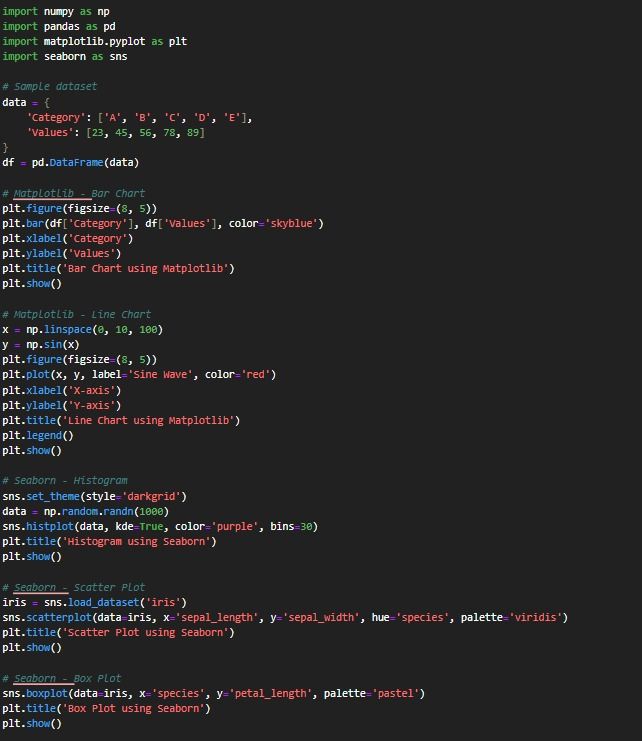
\includegraphics[width=14cm,height=12.3cm]{Matplotlib.jpeg}

\textbf{Output}:

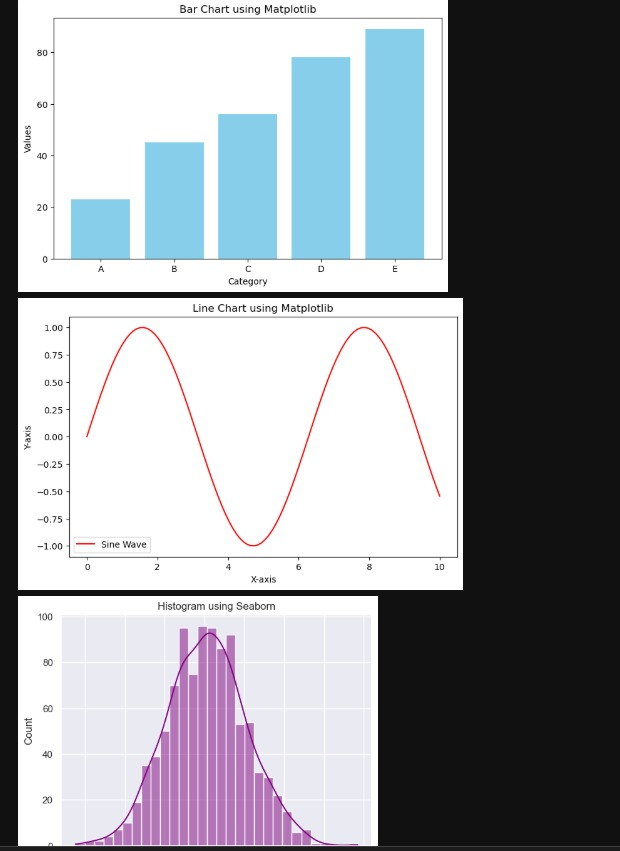
\includegraphics[width=14cm,height=12cm]{Matplotlib_Output.jpeg}

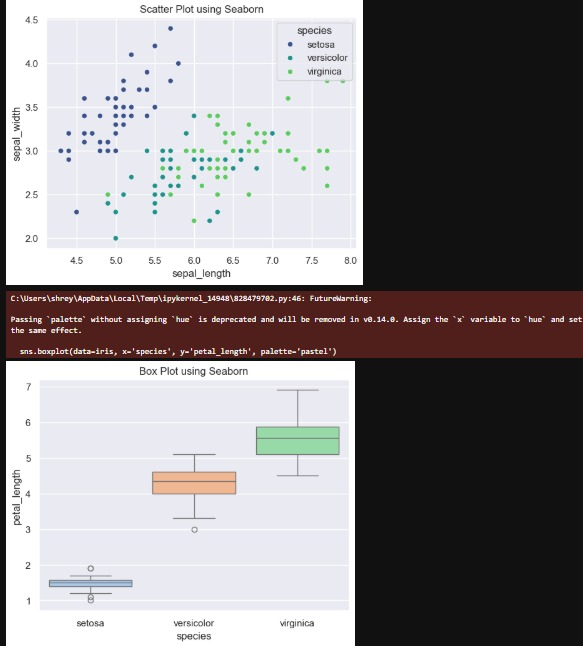
\includegraphics[width=14cm,height=12cm]{Matplotlib_Output2.jpeg}
\subsection{Scikit-Learn – Machine Learning}
\begin{itemize}
    \item Scikit-Learn is a popular machine learning library that offers easy and effective data mining and analysis tools.
    \item It is based on NumPy, SciPy, and Matplotlib and includes a variety of supervised and unsupervised learning algorithms.
    \item \textbf{Major Features}:
    \begin{itemize}
    \item Classification, regression, and clustering algorithms.
    \item Dimensionality reduction techniques.
    \item Model evaluation and hyperparameter tuning.
    \item Feature extraction and preprocessing utilities.
    \end{itemize}
\end{itemize}
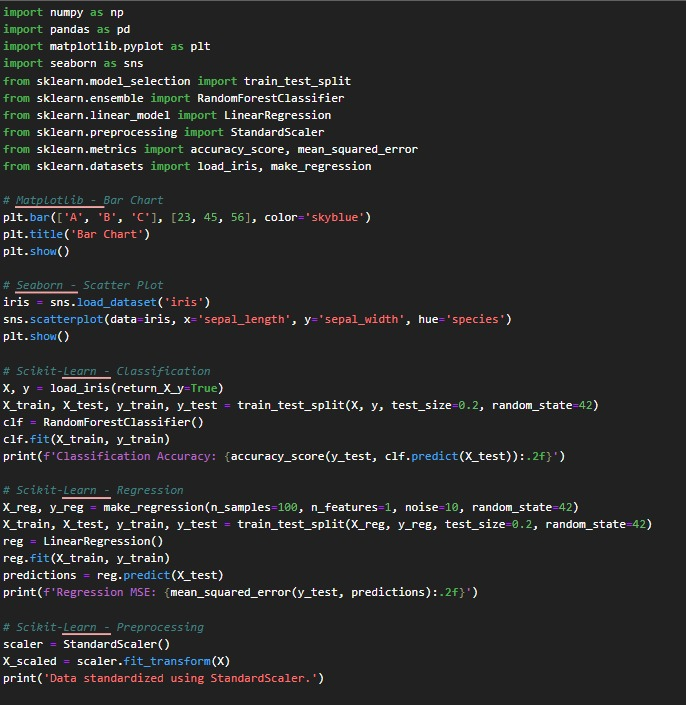
\includegraphics[width=14cm,height=10
cm]{Scikit.jpeg}

\textbf{Output}:

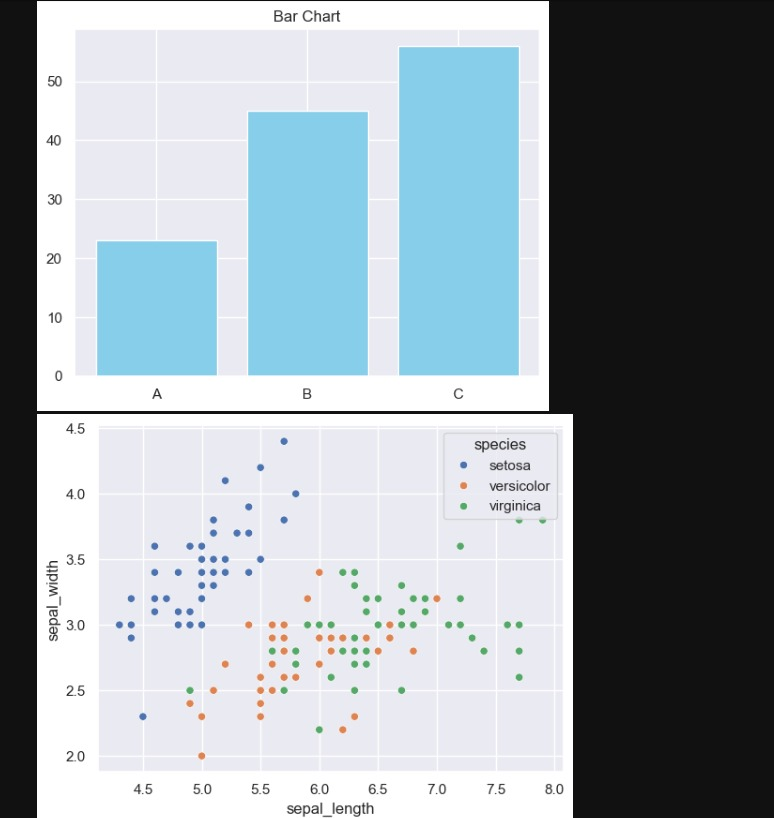
\includegraphics[width=14cm,height=8
cm]{Scikit_Output.jpeg}
\newpage
\subsection{Statsmodels – Statistical Modeling}
\begin{itemize}
    \item Statsmodels is a library intended for statistical hypothesis testing and modeling.
    \item It offers the functionality for performing statistical tests as well as for estimating statistical models.
    \item \textbf{Main Features}:
    \begin{itemize}
    \item Regression models (linear regression, logistic regression, and generalized linear models).
    \item Time series analysis.
    \item Hypothesis testing and statistical inference.
    \item Support for econometric models that are advanced.
    \end{itemize}
\end{itemize}
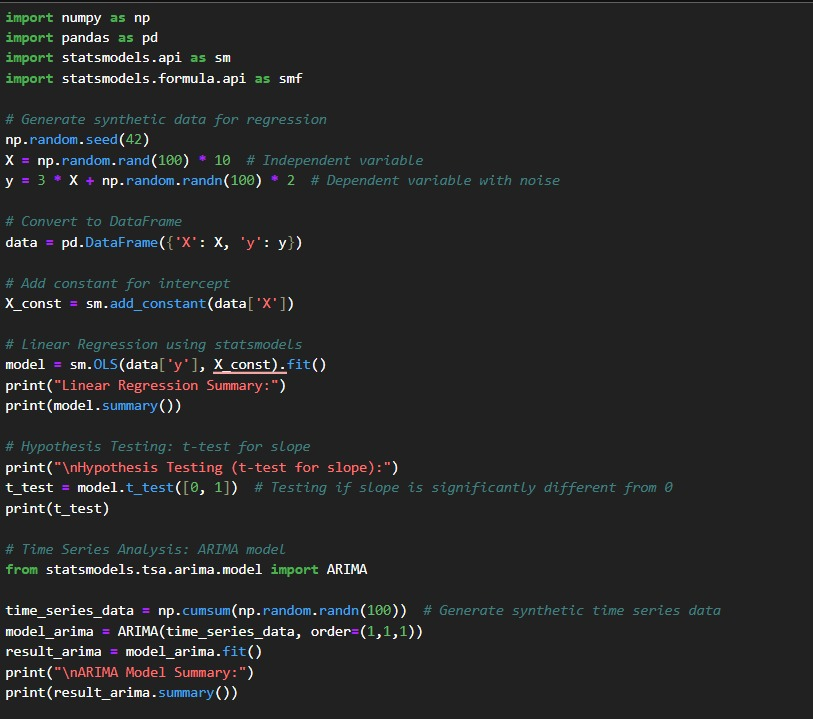
\includegraphics[width=14cm,height=10
cm]{Statsmodel.jpeg}

\textbf{Output}:

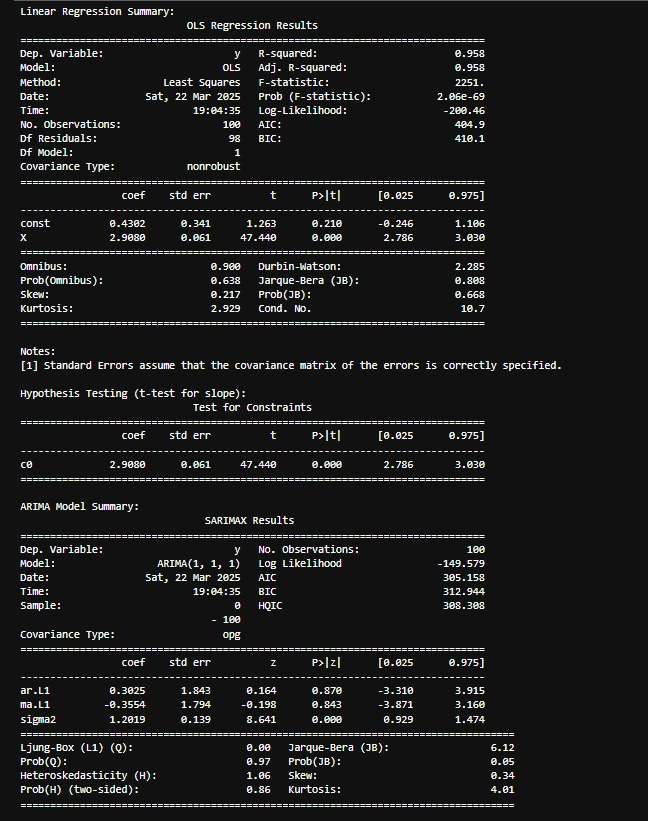
\includegraphics[width=14cm,height=9
cm]{Statsmodel_Output.jpeg}
\newpage
\subsection{SciPy – Advanced Mathematical Functions}
\begin{itemize}
    \item SciPy is an extension of the NumPy package with more functions for scientific and technical computing.
    \item It has modules for optimization, integration, interpolation, and signal processing.
    \item \textbf{Important Features}:
    \begin{itemize}
    \item Optimization and root-finding routines.
    \item Signal and image processing algorithms.
    \item Numerical integration and interpolation.
    \item Linear algebra and statistical operations.
    \end{itemize}
\end{itemize}
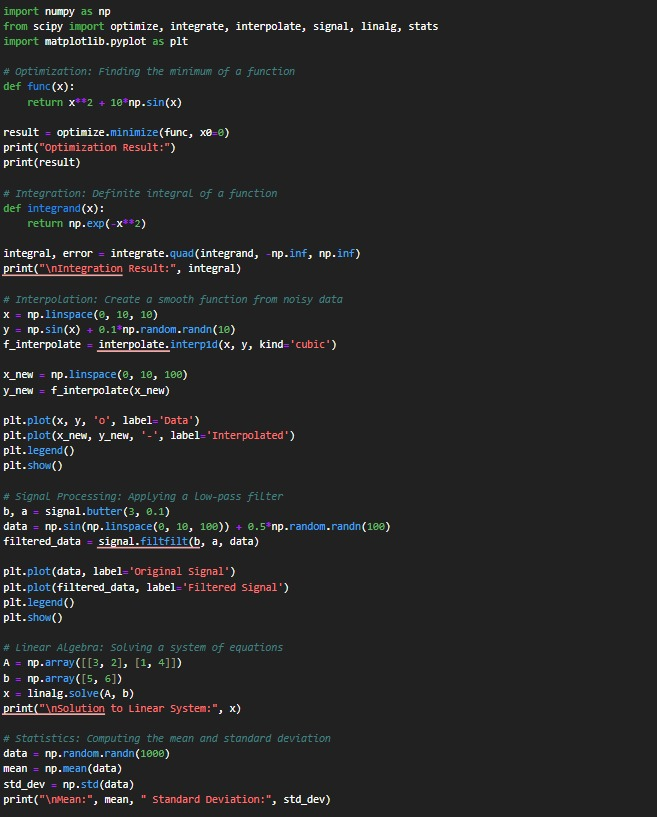
\includegraphics[width=14cm,height=18
cm]{SciPy.jpeg}
\newpage
\textbf{Output}:

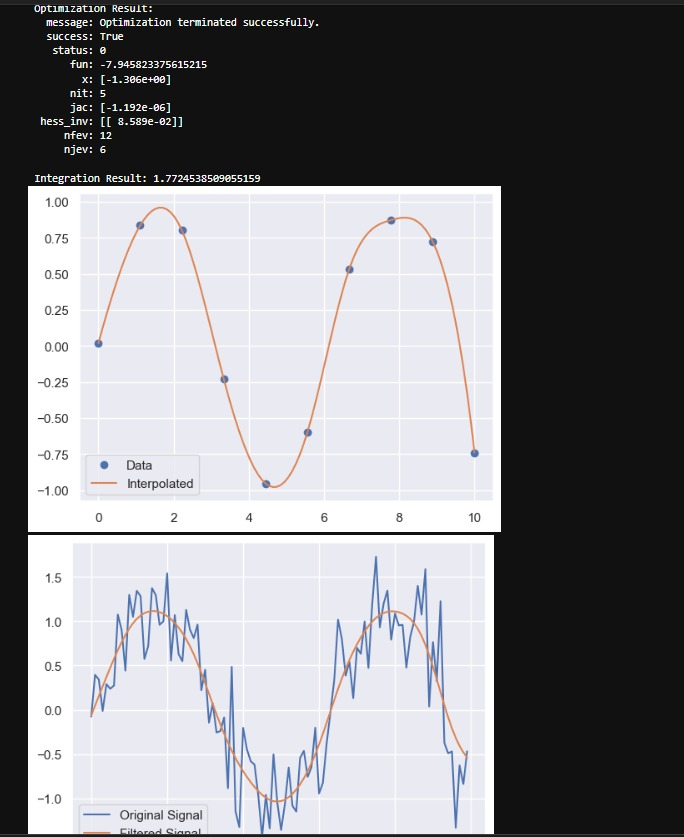
\includegraphics[width=14cm,height=20
cm]{SciPy_Output.jpeg}
\newpage
\subsection{Dask \& Vaex – Big Data Processing}
\begin{itemize}
    \item Dask and Vaex are specialized libraries for managing large datasets that are beyond the in-memory scope.
    \item Dask supports parallel computation for scalable data processing, and Vaex supports fast, out-of-core DataFrame manipulation.
\item \textbf{Important Features}:
    \begin{itemize}
    \item Dask: Parallel computation, lazy evaluation, and Pandas and NumPy integration.
    \item Vaex: Handling of large datasets with efficiency without loading them into memory.
    \item Support for distributed computing.
    \item Faster performance for big data analytics.
    \end{itemize}
\end{itemize}

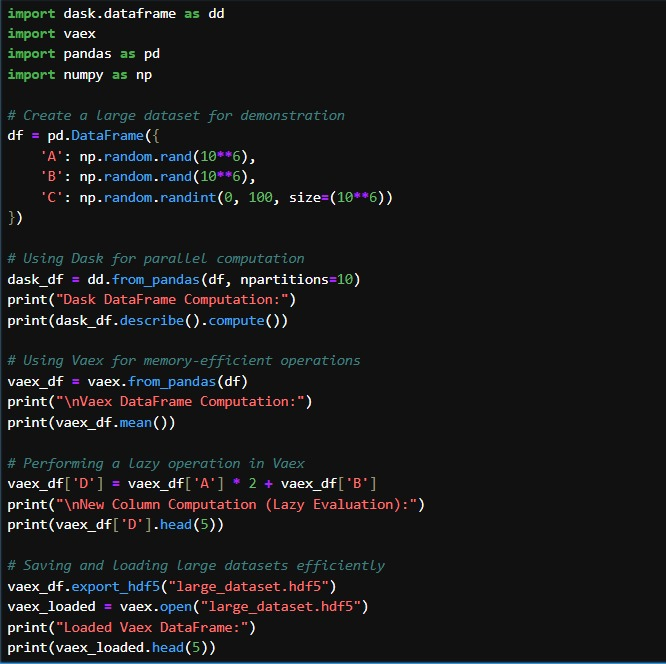
\includegraphics[width=14cm,height=18
cm]{Dask&Vaex.jpeg}
\newpage
\textbf{Output}:

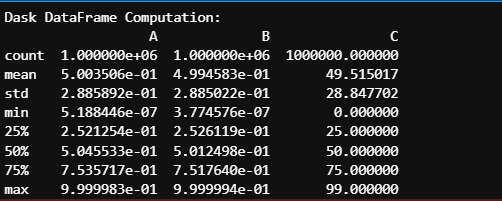
\includegraphics[width=14cm,height=6
cm]{Dask&Vaex_Output.jpeg}
\newpage
\section{Data Acquisition \& Processing}
Successful data acquisition and processing are essential phases in any data science process. This chapter discusses some of the approaches to acquiring, cleaning, and converting data for high-quality inputs into analysis and machine learning models.
\subsection {Reading and Writing Data}
\begin{itemize}
    \item Efficient reading and writing of data is required to work with structured and unstructured data sets.
    \item Python offers a number of libraries to read and write various file formats like CSV, JSON, Excel, and databases.
    \item \textbf{Important Functions}:
    \begin{itemize}
    \item pandas.read\_csv(), pandas.to\_csv() for CSV.
    \item pandas.read\_excel(), pandas.to\_excel() for Excel.
    \item json.load(), json.dump() for JSON.
    \item SQL database operations using sqlite3 or SQLAlchemy.
    \end{itemize}
    
\end{itemize}

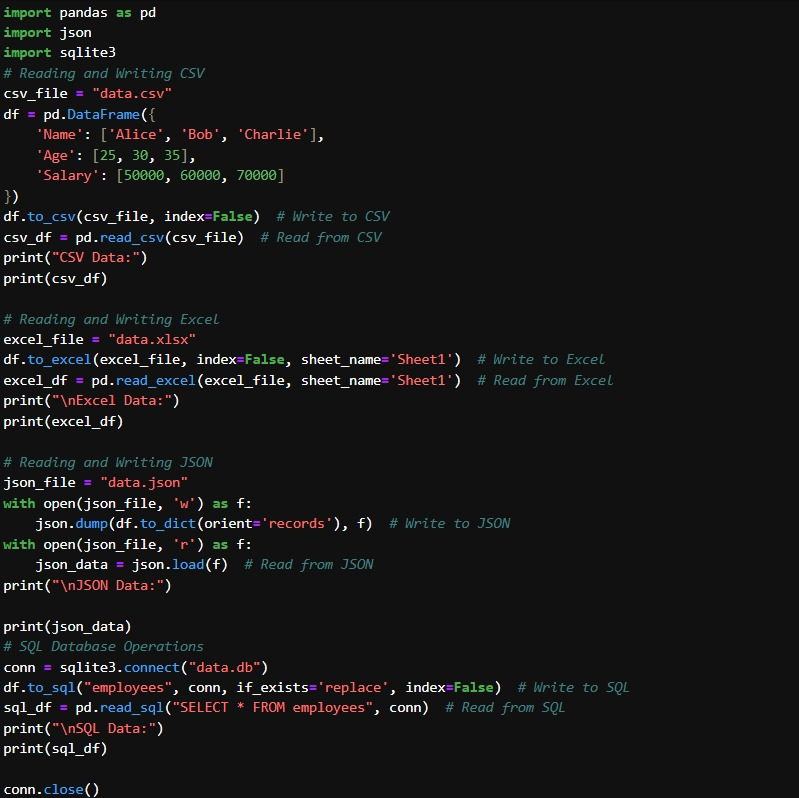
\includegraphics[width=14cm,height=16
cm]{Reading&Writing.jpeg}

\textbf{Output}:

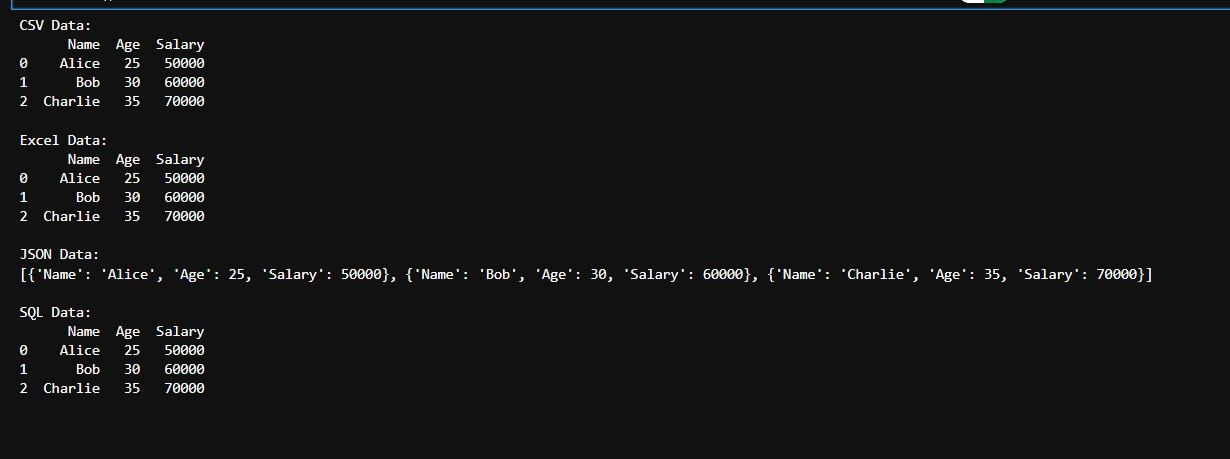
\includegraphics[width=14cm,height=6.5
cm]{Reading&Writing_Output.jpeg}
\subsection {Web Scraping}
\begin{itemize}
    \item Web scraping enables data gathering from websites with automated programs.
    \item Python offers BeautifulSoup and Scrapy libraries for efficiently scraping and parsing web pages.
    \item \textbf{Important Methods}:
    \begin{itemize}
    \item Parsing HTML using BeautifulSoup.
    \item Automating requests with requests and urllib.
    \item Gathering structured data using Scrapy.
    \item Processing JavaScript-rendered content with Selenium.
    \end{itemize}
\end{itemize}

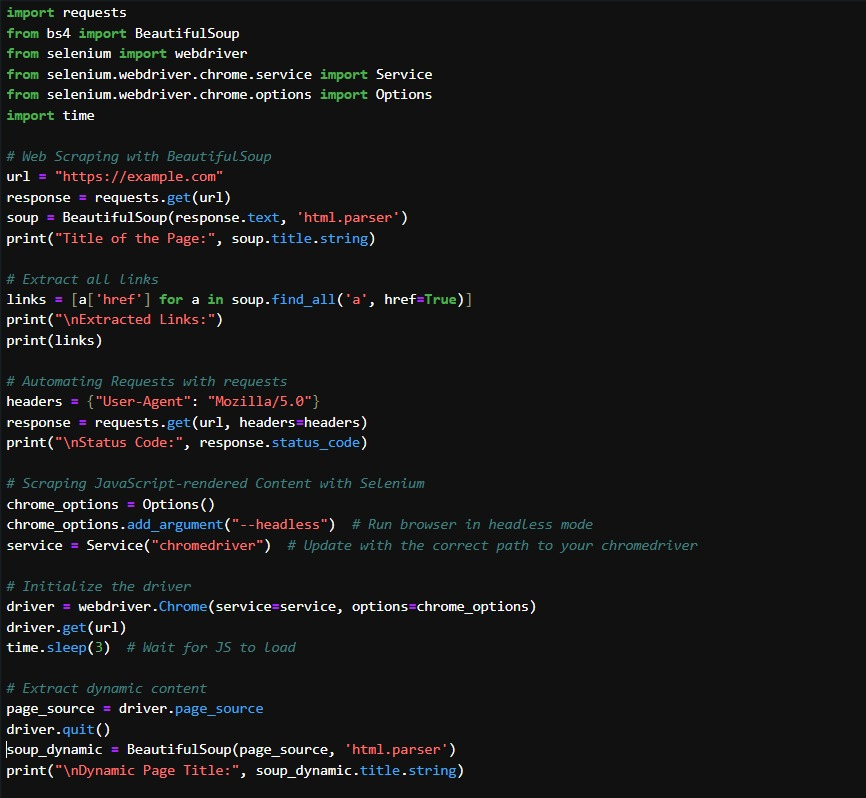
\includegraphics[width=14cm,height=12
cm]{WebScraping.jpeg}

\textbf{Output}:


\includegraphics[width=14cm,height=4
cm]{WebScraping_Output.jpeg}
\subsection{Working with APIs}
\begin{itemize}
    \item APIs (Application Programming Interfaces) provide data retrieval from external sources like social media websites, financial data providers, and open data stores.
    \item \textbf{Important Methods}:
    \begin{itemize}
    \item Utilizing requests to retrieve data from REST APIs.
    \item Authentication handling with API keys or OAuth.
    \item Processing JSON responses with json library.
    \item Working with third-party services like Twitter API, OpenWeather API, and Google Maps API.
    \end{itemize}
\end{itemize}
\subsection{Handling Missing Values and Outliers}
\begin{itemize}
    \item Managing missing values and outliers is important for data quality and avoiding biases in analysis and machine learning models.
\item \textbf{Important Methods}:
    \begin{itemize}
    \item Finding missing values with pandas.isnull().
    \item Replacing missing values with mean, median, or mode with fillna().
    \item Identifying and removing outliers through statistical measures (e.g., Z-score, IQR).
    \item Advanced imputation techniques with sklearn.impute.
    \end{itemize}
\end{itemize}
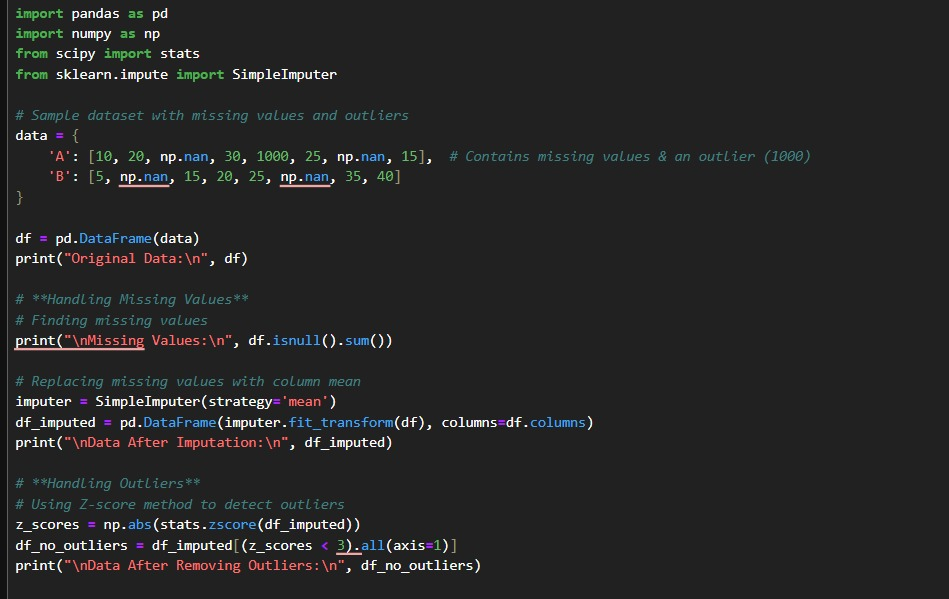
\includegraphics[width=14cm,height=12
cm]{HandlingMissing.jpeg}

\textbf{Output}:

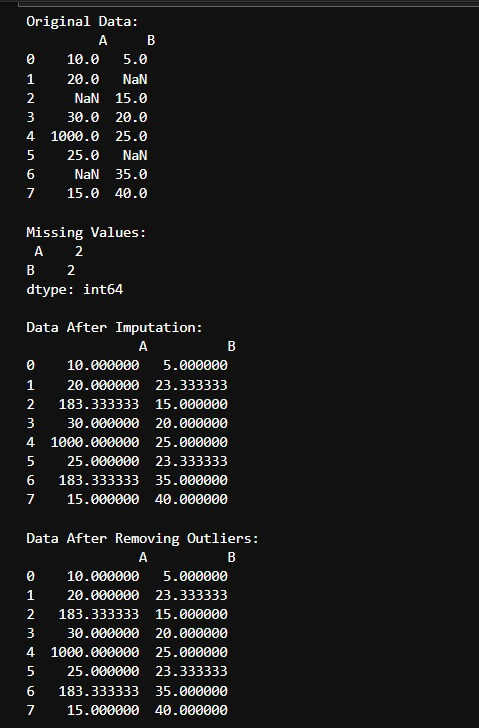
\includegraphics[width=14cm,height=4
cm]{HandlingMissing_Output.jpeg}
\newpage
\subsection{Feature Engineering and Transformation}  
\begin{itemize}
    \item Feature engineering is about developing new features or feature transformations to best enhance model performance.
    \item Optimal predictive precision relies on it.
\item \textbf{Important Methods}:
    \begin{itemize}
    \item Categorical variable encoding (label encoding, one-hot encoding).
    \item Scaling numerical features using StandardScaler, MinMaxScaler.
    \item Polynomial feature generation with PolynomialFeatures.
    \item Principal Component Analysis (PCA) dimensionality reduction.
    \item Creating interaction features to pick up interactions between variables.
    \end{itemize}
\end{itemize}

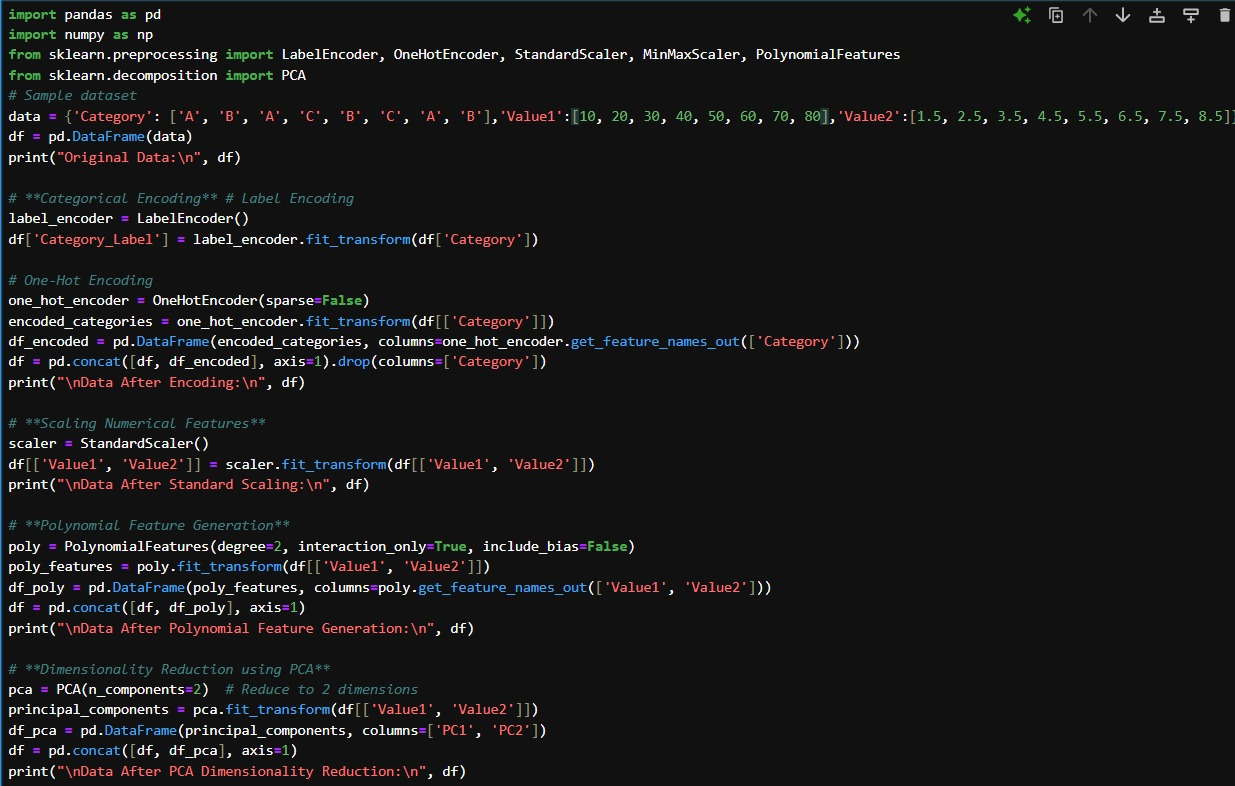
\includegraphics[width=17cm,height=14
cm]{FeatureEngineering.jpeg}

\textbf{Output}:

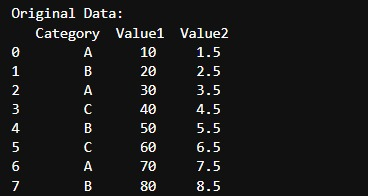
\includegraphics[width=14cm,height=4
cm]{FeatureEngineering_Output.jpeg}


\newpage
\section{Exploratory Data Analysis (EDA)}
Exploratory Data Analysis (EDA) is a key process for discovering the inherent patterns and structures in a dataset. It consists of summarizing, visualizing, and changing data to infer useful information.
\subsection{Summary Statistics}
\begin{itemize}
    \item Summary statistics give a rapid overview of the dataset to reveal trends, distributions, and possible problems.
    \item \textbf{Important Methods}:
    \begin{itemize}
    \item pandas.describe() for numerical summaries.
    \item pandas.info() for structure of the dataset.
    \item Calculation of mean, median, standard deviation, and percentiles.
    \item Grouping and summarizing data using groupby().
    \end{itemize}
\end{itemize}

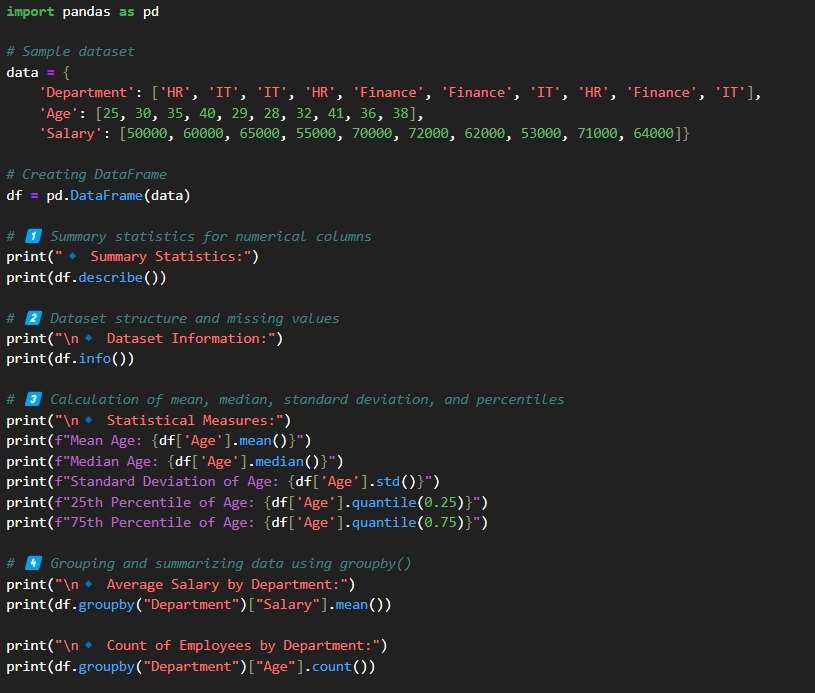
\includegraphics[width=17cm,height=16
cm]{Summary.jpeg}
\newpage
\textbf{Output}:

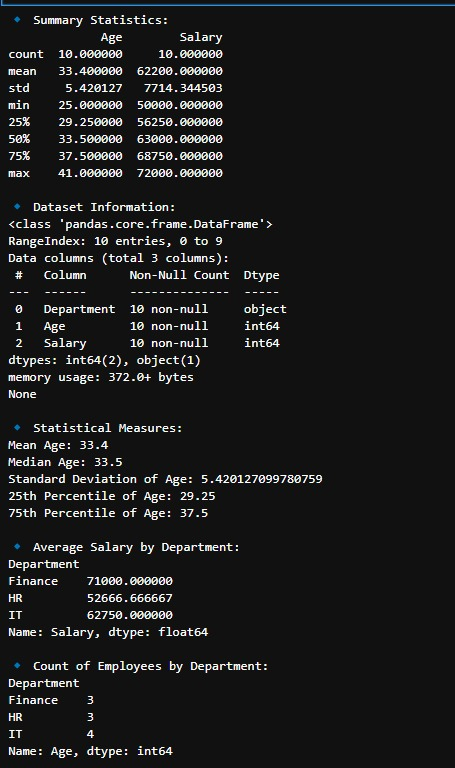
\includegraphics[width=14cm,height=18
cm]{Summary_Output.jpeg}
\subsection{Visualizing Distributions and Correlations}
\begin{itemize}
    \item Visualizing distributions and correlations of data assists in identifying patterns and relationships between variables.
\item \textbf{Important Methods}:
    \begin{itemize}
    \item Histograms and density plots with seaborn.histplot() and sns.kdeplot().
    \item Boxplots and violin plots for identifying outliers.
    \item Scatter plots and pair plots for relationships.
    \item Correlation heatmaps with sns.heatmap().
    \end{itemize}
\end{itemize}
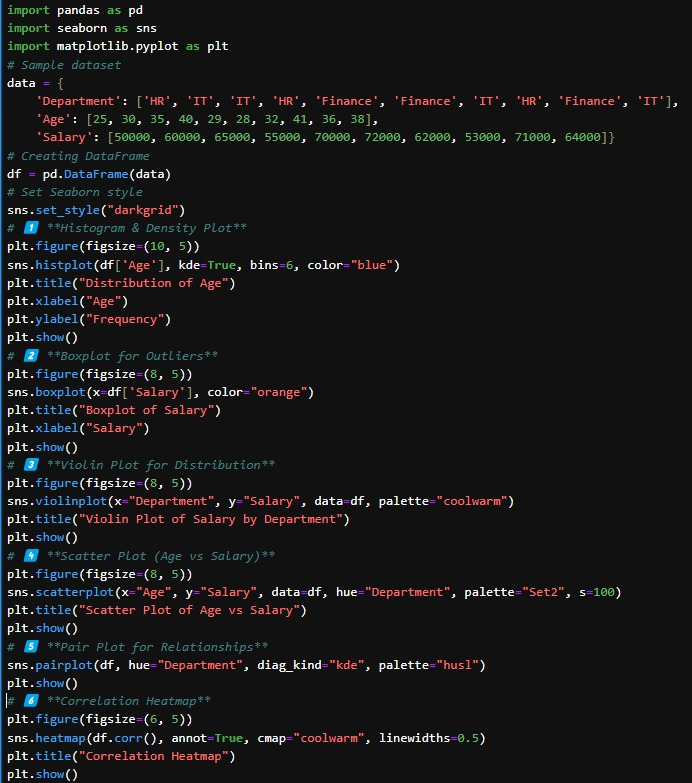
\includegraphics[width=17cm,height=20
cm]{Visualizing.jpeg}
\newpage
\textbf{Output}:

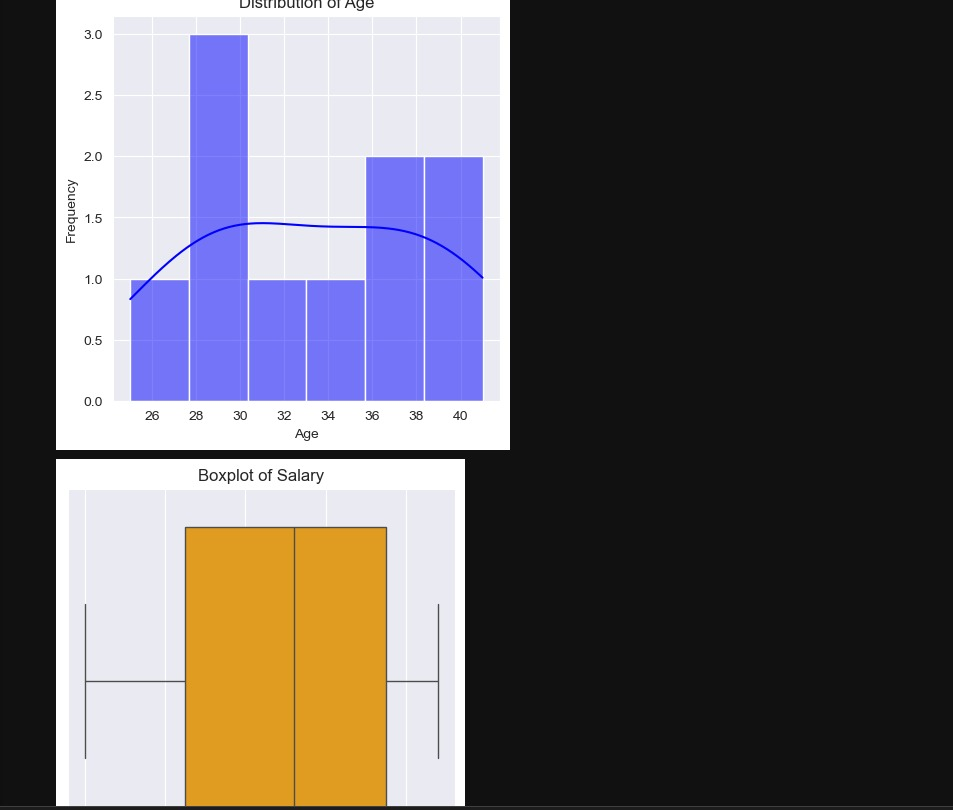
\includegraphics[width=14cm,height=10
cm]{Visualizing_Output.jpeg}

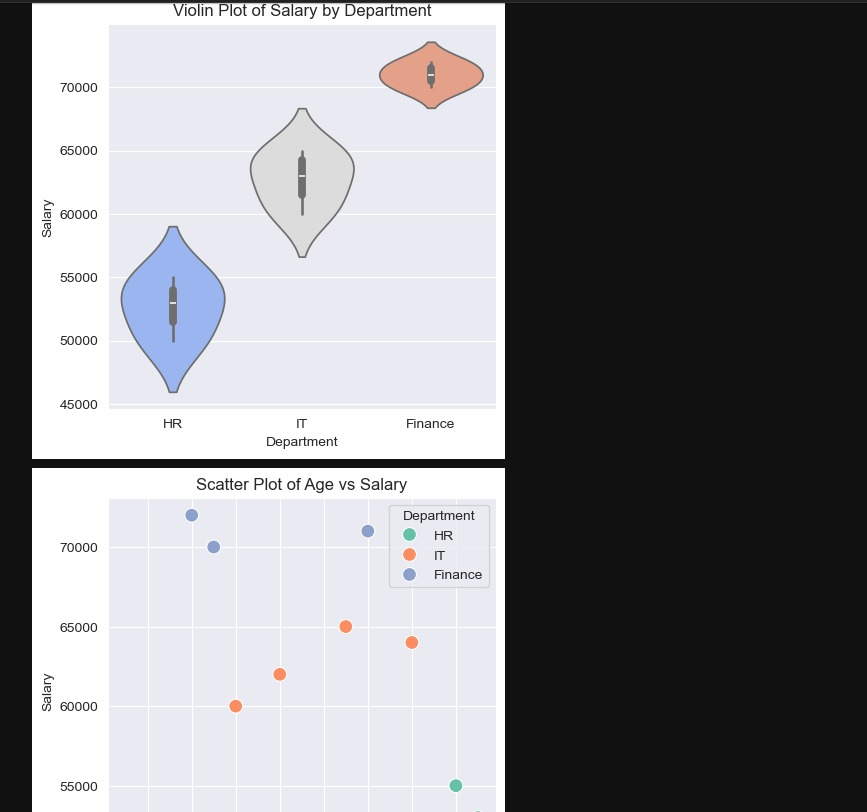
\includegraphics[width=14cm,height=10
cm]{Visualizing_Output2.jpeg}
\subsection{Dimensionality Reduction}
\begin{itemize}
    \item Dimensionality reduction methods assist in the simplification of datasets maintaining key information. 
    \item \textbf{Important Methods}:
    \begin{itemize}
    \item Principal Component Analysis (PCA).
    \item t-Distributed Stochastic Neighbor Embedding (t-SNE).
    \item Uniform Manifold Approximation and Projection (UMAP).
    \item Feature selection and feature extraction methods.
    \end{itemize}
\end{itemize}
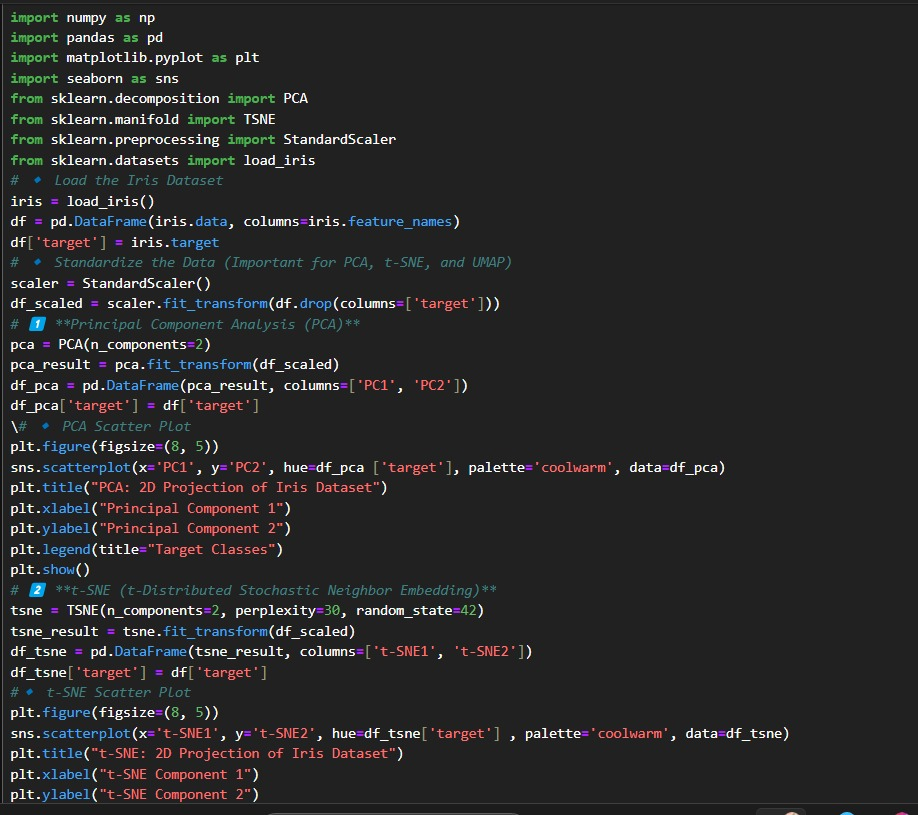
\includegraphics[width=17cm,height=20
cm]{Dimensionality Reduction.jpeg}
\newpage
\textbf{Output}:

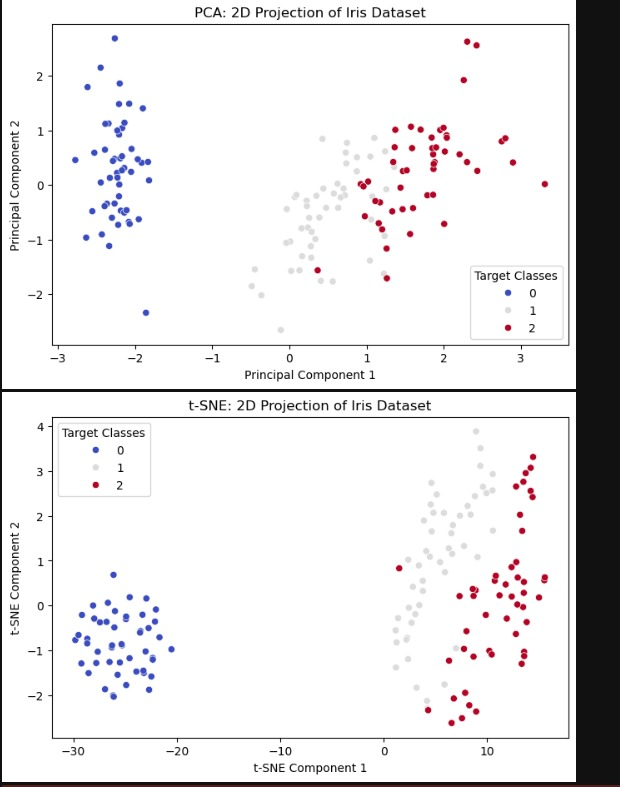
\includegraphics[width=14cm,height=12
cm]{Dimensionality Reduction_Output.jpeg}

\newpage
\section{Machine Learning with Python}
Machine learning allows computers to learn patterns from data and predict. Python offers a great set of libraries for constructing machine learning models. This section introduces important concepts and techniques applied in machine learning with Python.
\subsection{Supervised vs. Unsupervised Learning}
Machine learning is divided into two broad categories:
\begin{itemize}
    \item \textbf{Supervised Learning}: The model is trained on labeled data (input-output pairs) to predict. 
    
    \textbf{Example}: Classifying emails as spam or not spam.
    \item \textbf{Unsupervised Learning}: The model discovers patterns in unlabeled data without direct supervision.
    
    \textbf{Example}: Grouping customers based on purchasing behavior.
\end{itemize}
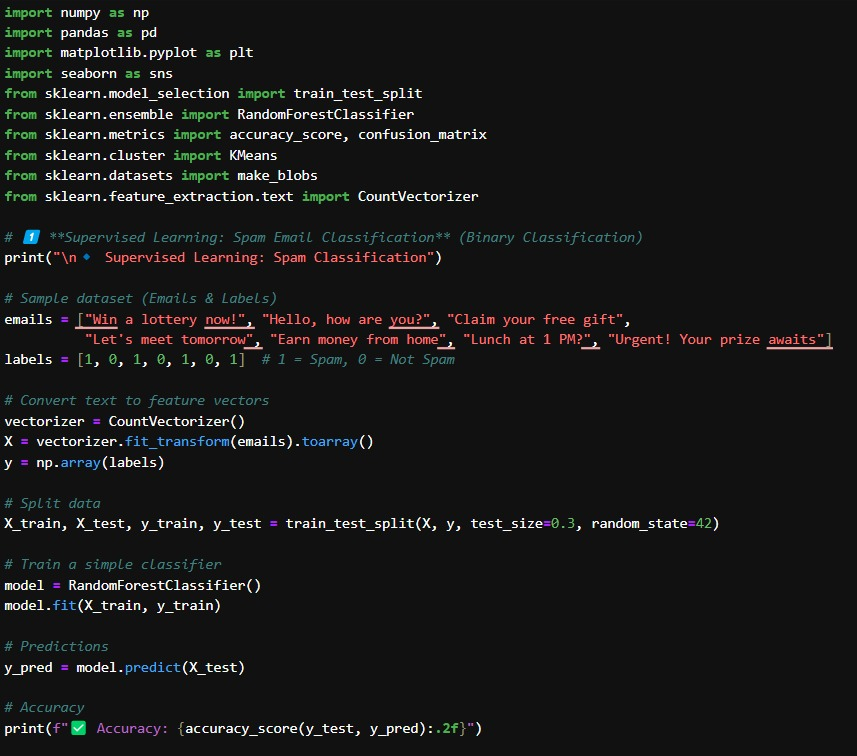
\includegraphics[width=16cm,height=14
cm]{Supervised.jpeg}

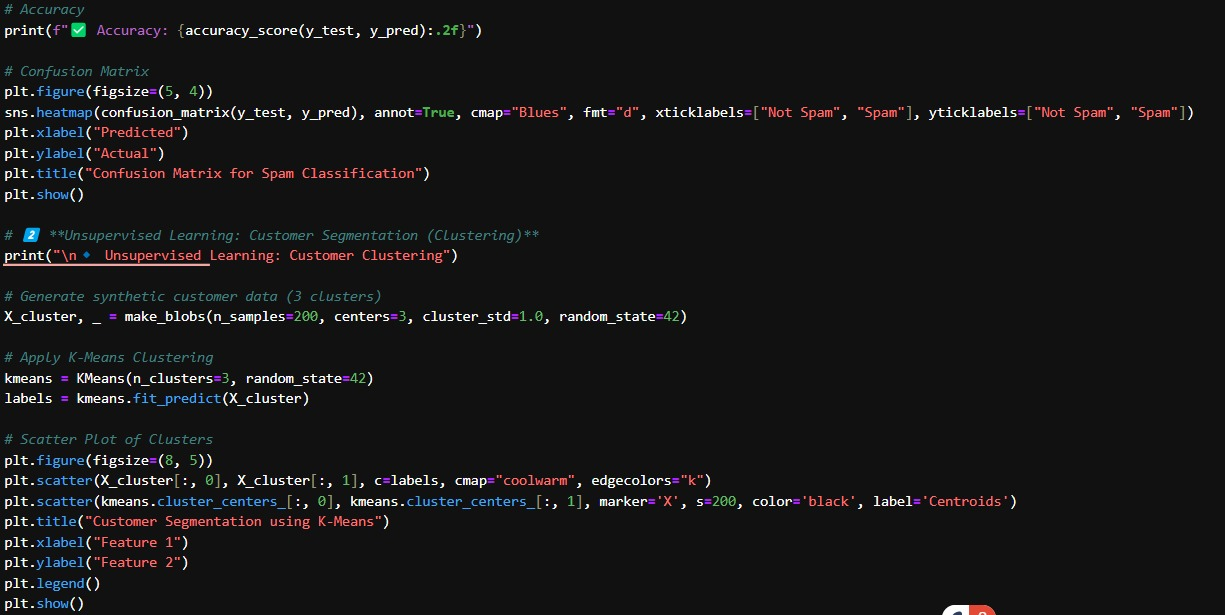
\includegraphics[width=16cm,height=12
cm]{Supervised2.jpeg}

\textbf{Output}:

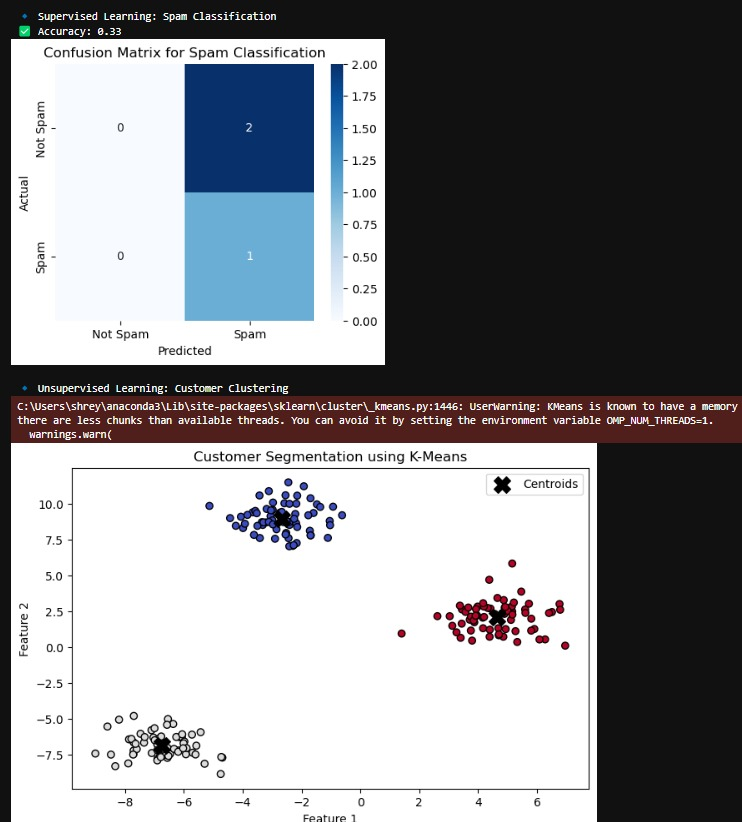
\includegraphics[width=16cm,height=12
cm]{Supervised_Output.jpeg}


\subsection{Regression}
\begin{itemize}
    \item Regression is a supervised learning technique applied in the process of predicting continuous values.
    \item It is also extensively utilized in forecasting and trend estimation.
    \item \textbf{Important Methods}:
    \begin{itemize}
    \item \textbf{Linear Regression}: Applies regression on linear relationship between target variable and input variables.
    
    \textbf{Example}: Predicting house prices based on square footage.

    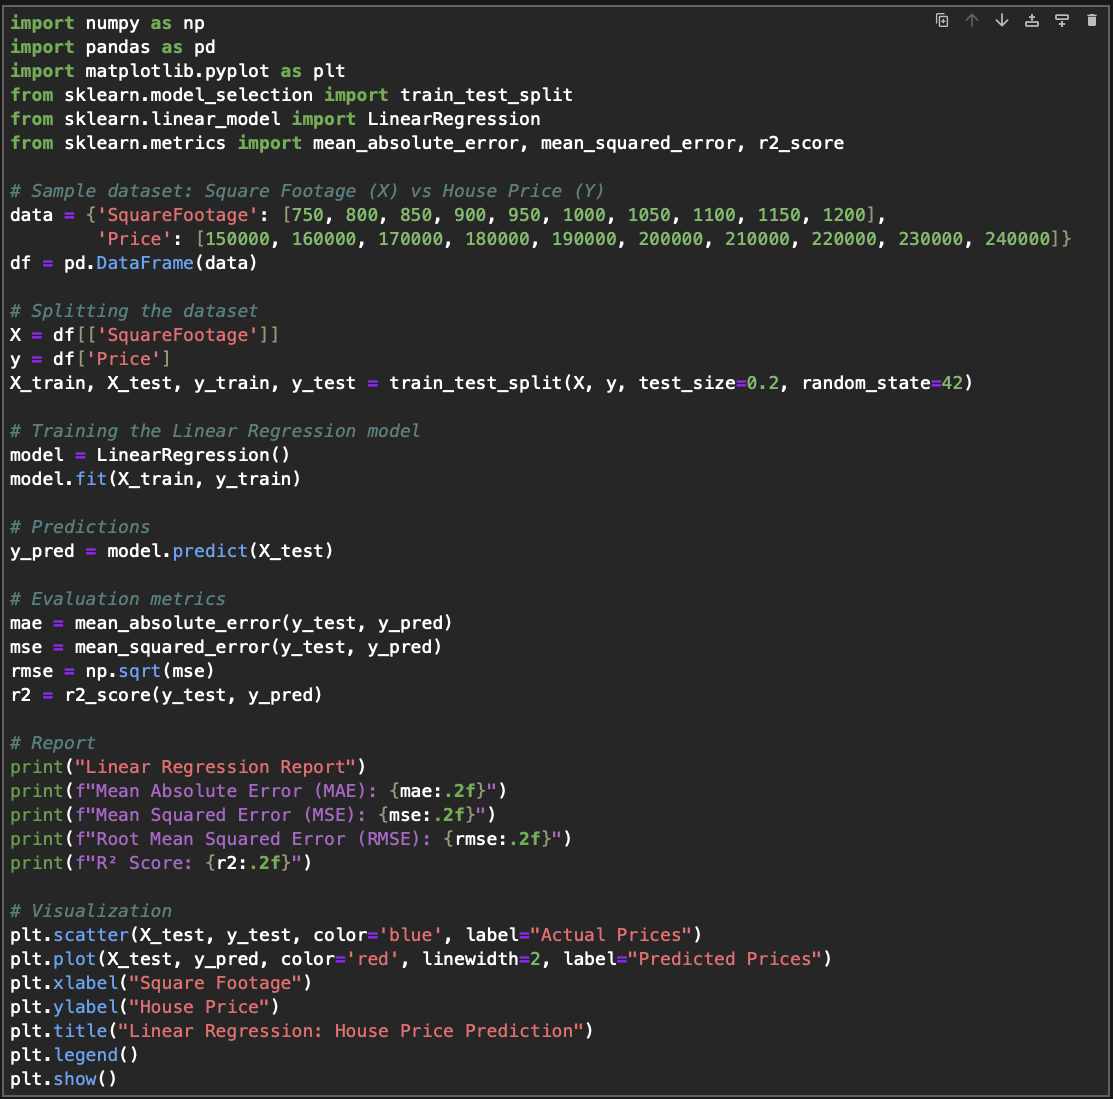
\includegraphics[width=14cm,height=14cm]{Linear.png}

\textbf{Output}:

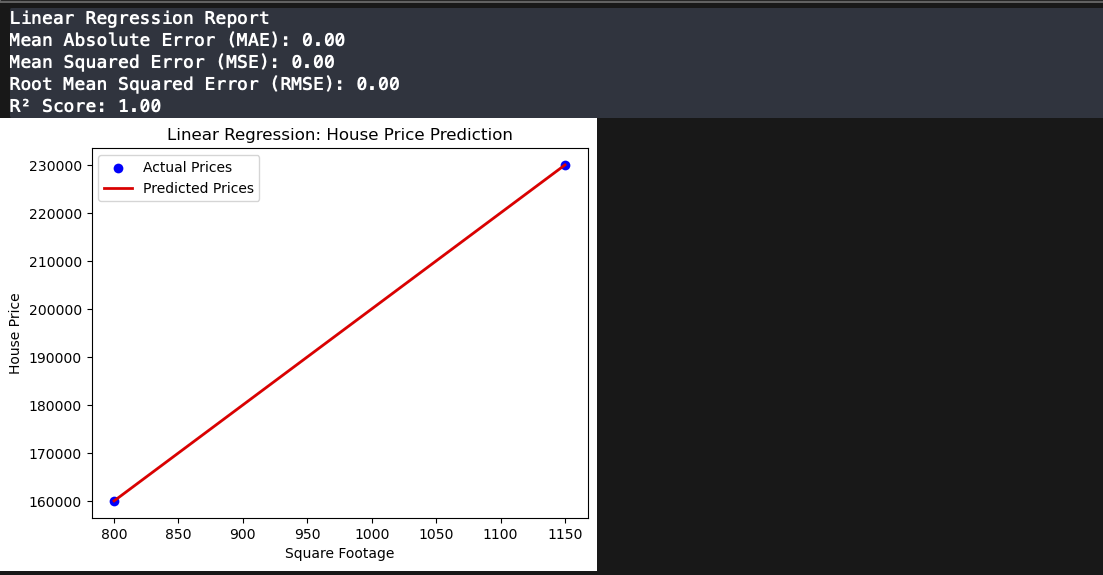
\includegraphics[width=14cm,height=6
cm]{Linear_Output.png}
    \item \textbf{Polynomial Regression}: An extension of linear regression for application in dealing with non-linearity.
    
    \textbf{Example}: Predicting car price based on age and mileage with a curved trend.

    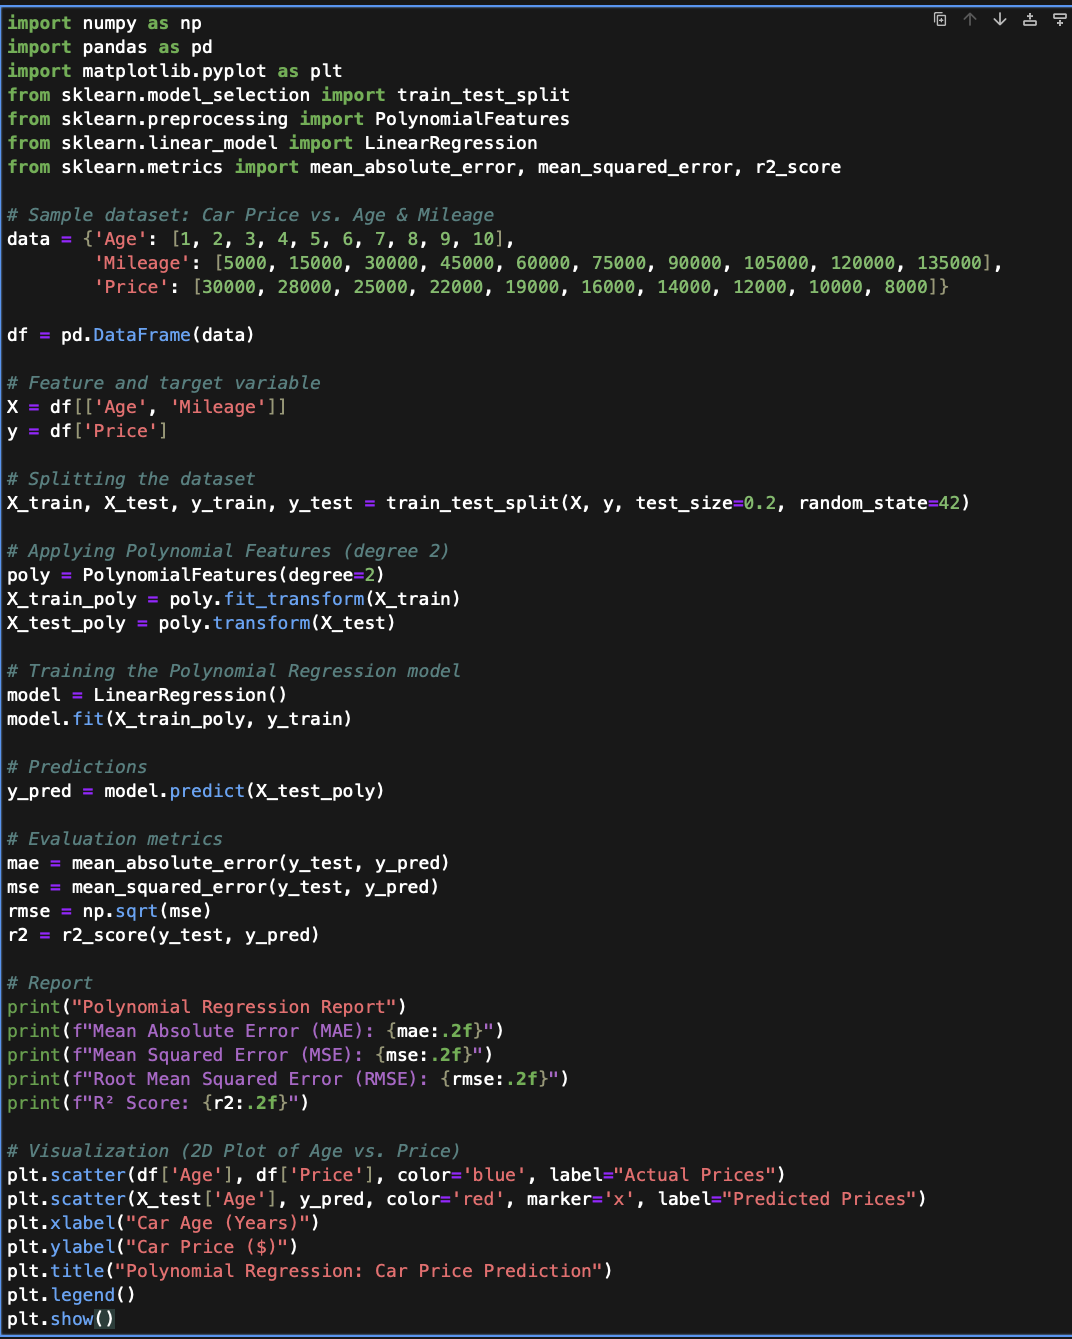
\includegraphics[width=14cm,height=14cm]{Polynomial Regression.png}

\textbf{Output}:

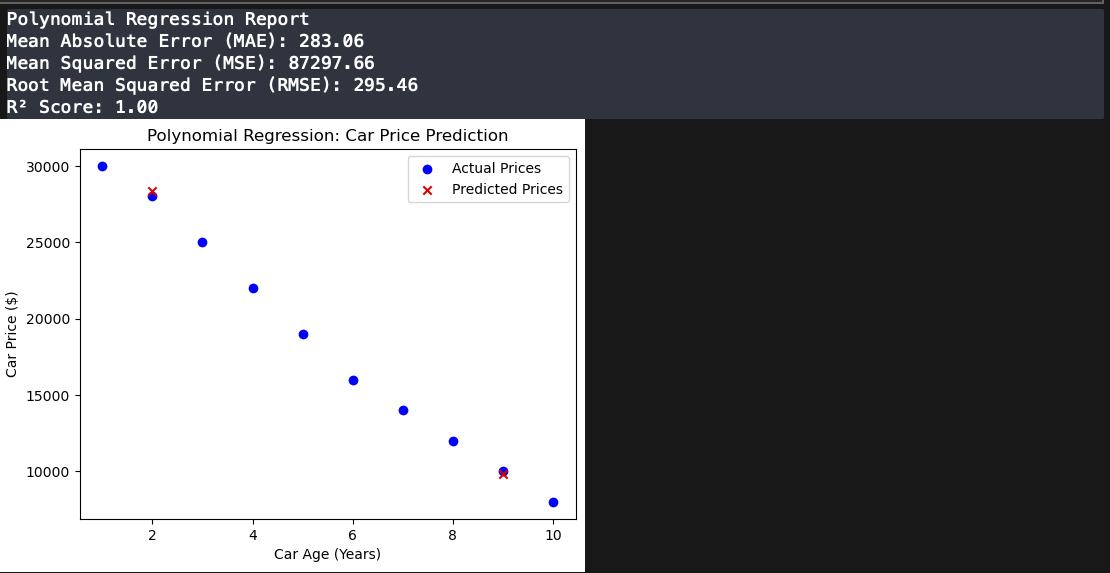
\includegraphics[width=14cm,height=6
cm]{Polynomial Regression_Output.png}
    \item \textbf{Ridge and Lasso Regression}: Introduces regularization for the intention of avoiding overfitting. 
    
    \textbf{Example of Ridge Regression}: Predicting house prices while reducing the impact of less important features
    
    \textbf{Example of Lasso Regression}: Predicting house prices while automatically selecting the most relevant features.

    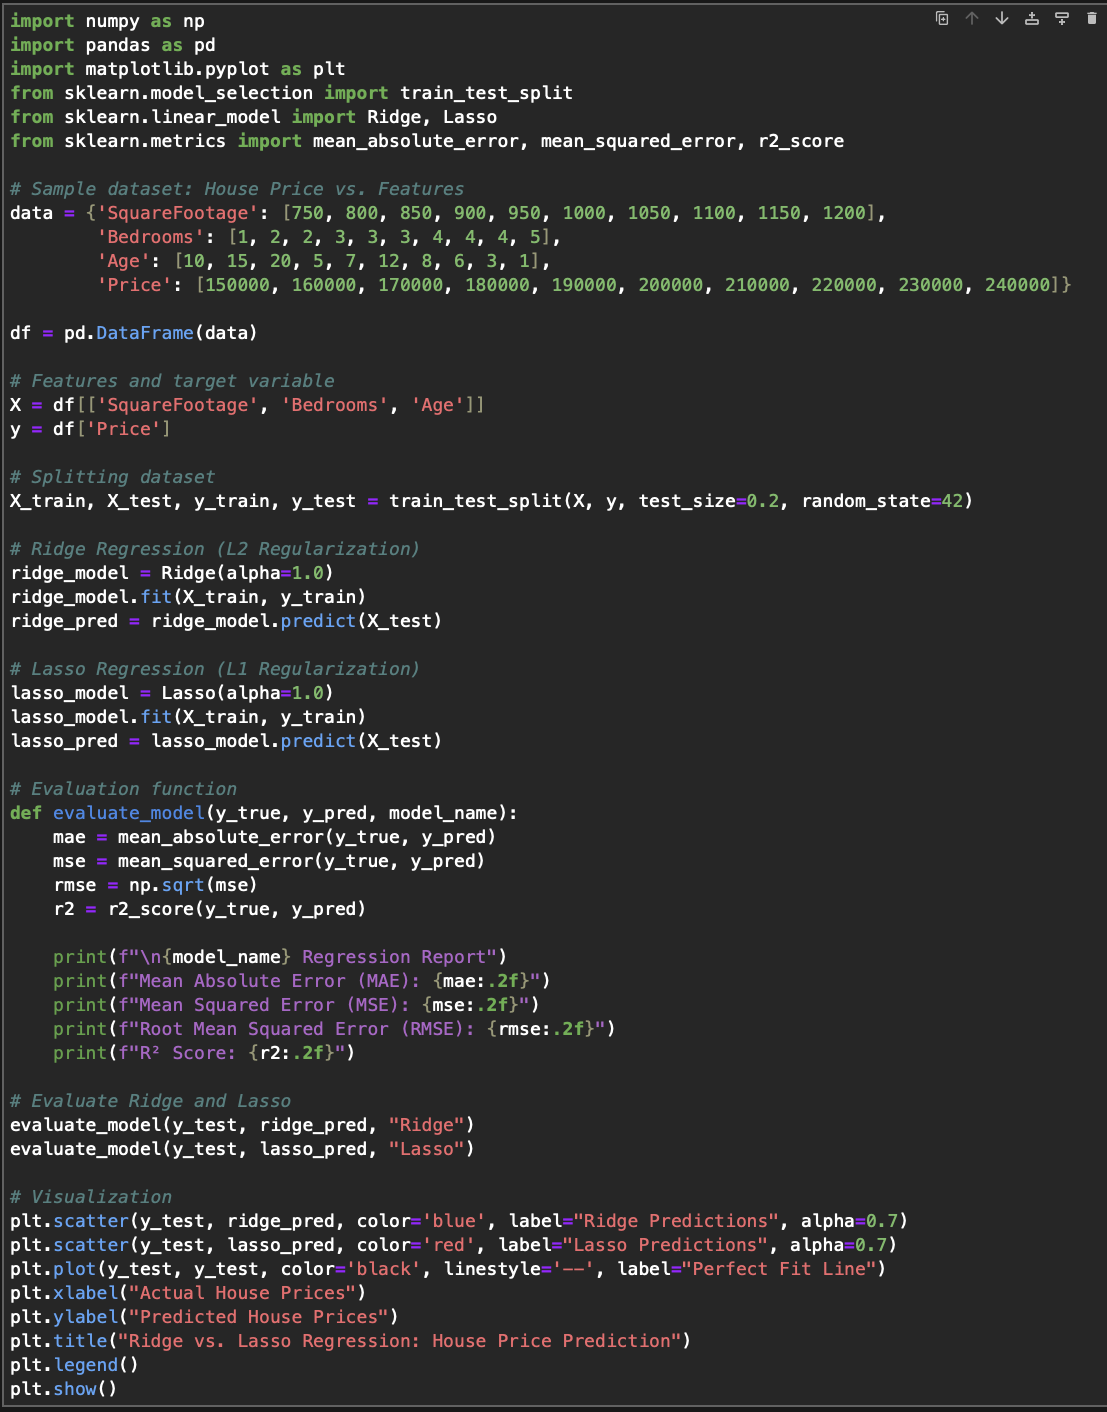
\includegraphics[width=14cm,height=14cm]{Ridge .png}

\textbf{Output}:

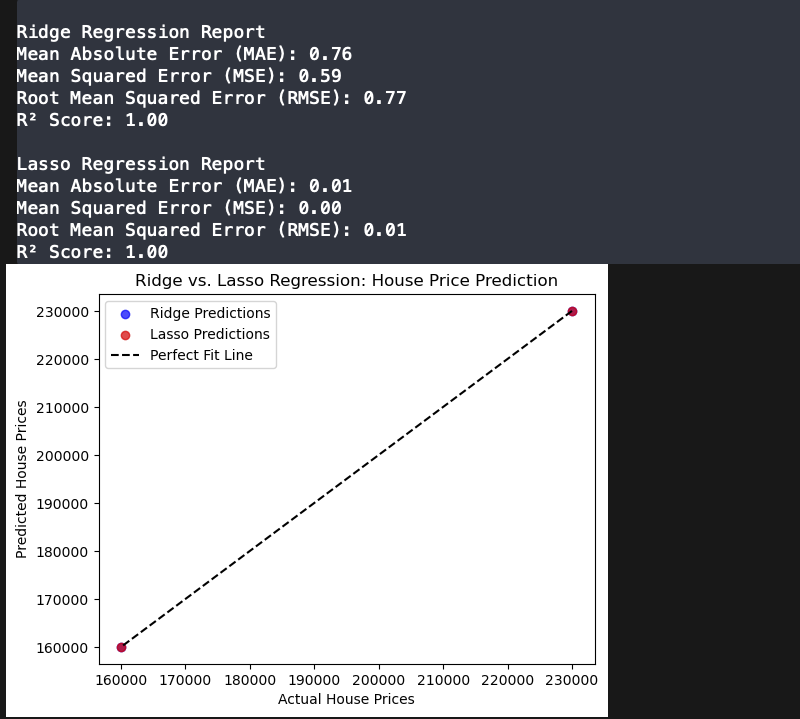
\includegraphics[width=14cm,height=8
cm]{Ridge _Output.png}
    \item \textbf{Decision Tree and Random Forest Regression}: Non-linear techniques for managing complex relationships.

    \textbf{Example of Decision Tree Regression}: Predicting house prices by splitting data based on features like location and size.

    \textbf{Example of Random Forest Regression}: Improving house price predictions by averaging multiple decision trees.

    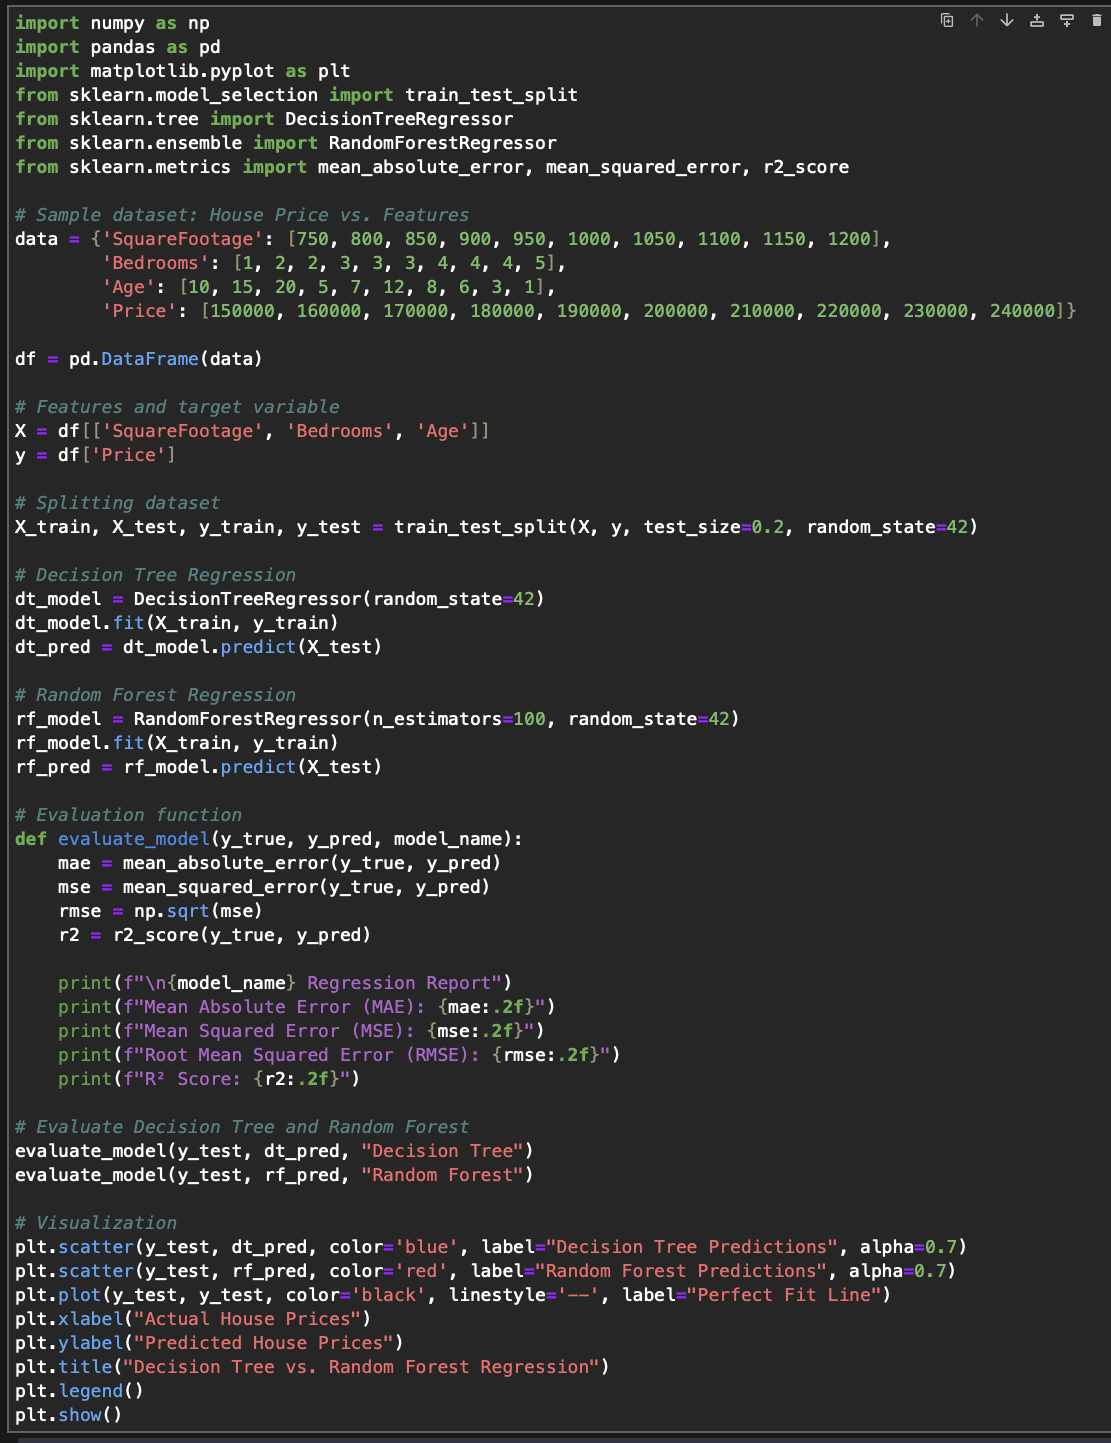
\includegraphics[width=14cm,height=18cm]{Forest Regression.png}

\newpage
\textbf{Output}:

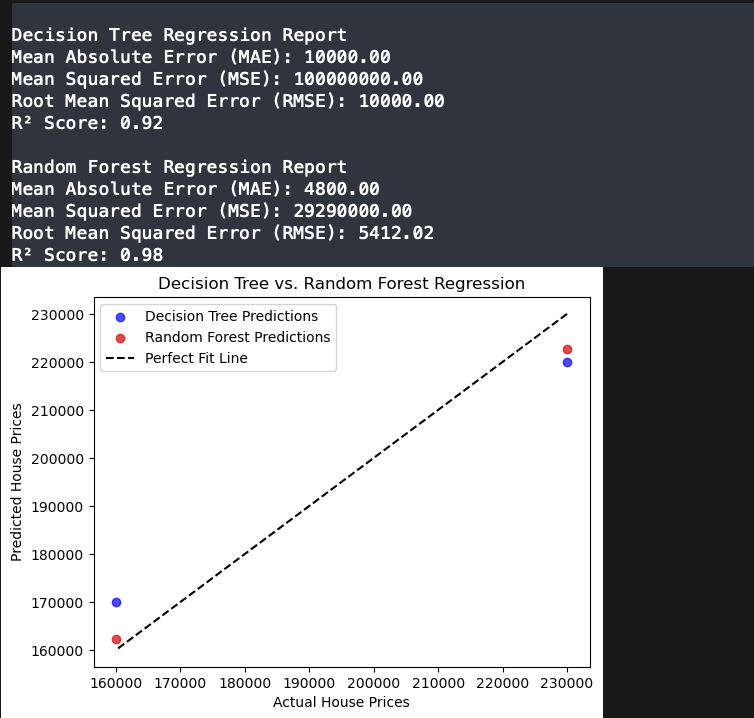
\includegraphics[width=14cm,height=6.5
cm]{Forest Regression_Output.png}
    \item \textbf{Support Vector Regression (SVR)}: Uses kernel functions to map input data into high-dimensional spaces.

    \textbf{Example}: Predicting stock prices by fitting the best boundary within a margin.

    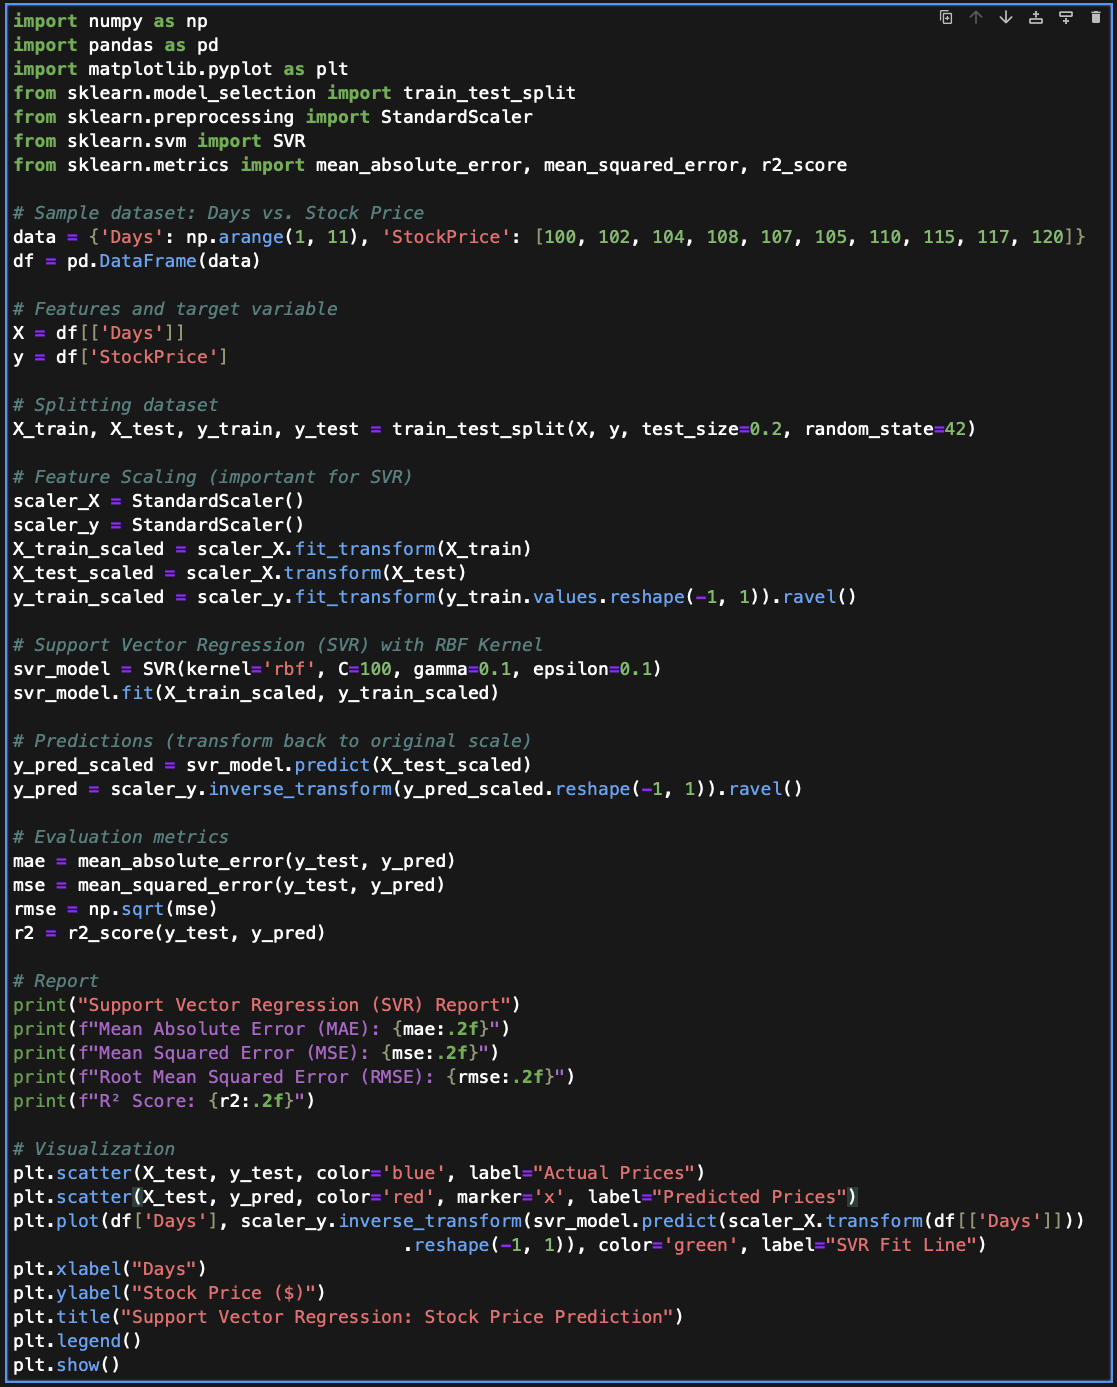
\includegraphics[width=14cm,height=16cm]{SVR.png}

\newpage
\textbf{Output}:

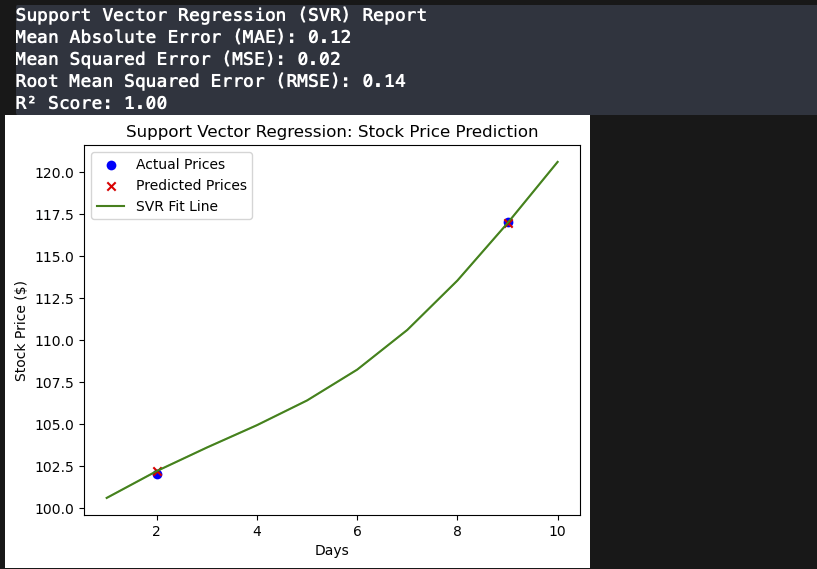
\includegraphics[width=14cm,height=6
cm]{SVR_Output.png}
    \end{itemize}
\end{itemize}
\subsection{Classification}
\begin{itemize}
    \item Classification is a supervised learning issue where categorical decisions need to be made.
    \item \textbf{Important Methods}:
    \begin{itemize}
    \item \textbf{Logistic Regression}: For problems in binary classification.

    \textbf{Example}: Predicting whether a customer will buy a product (Yes/No).

    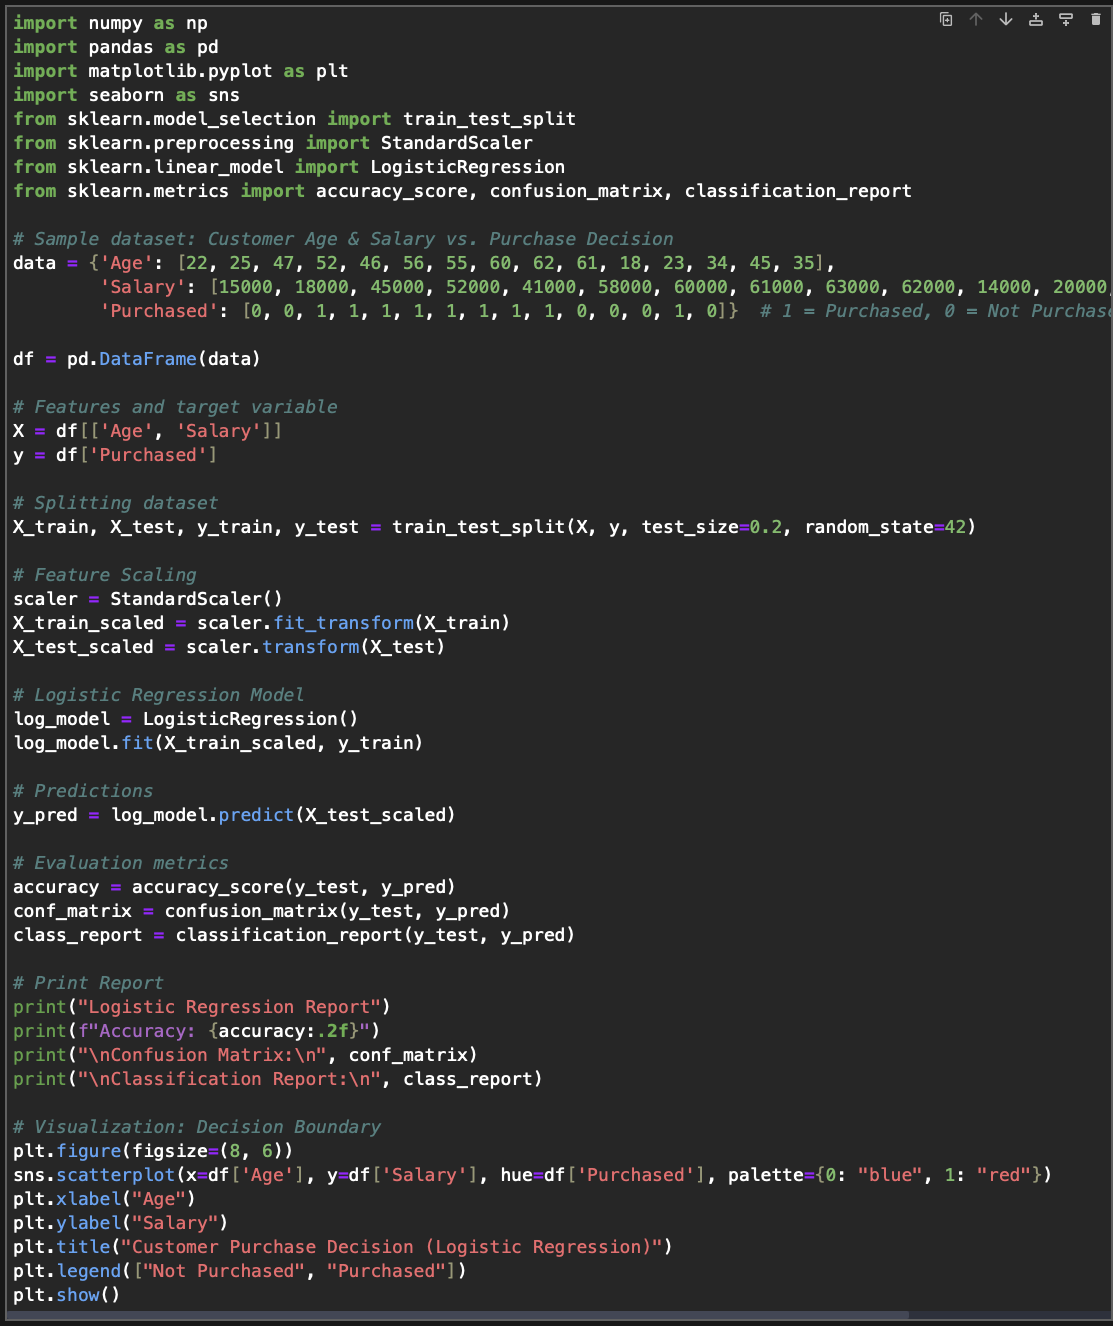
\includegraphics[width=14cm,height=14.5cm]{Logistic .png}

\newpage
\textbf{Output}:

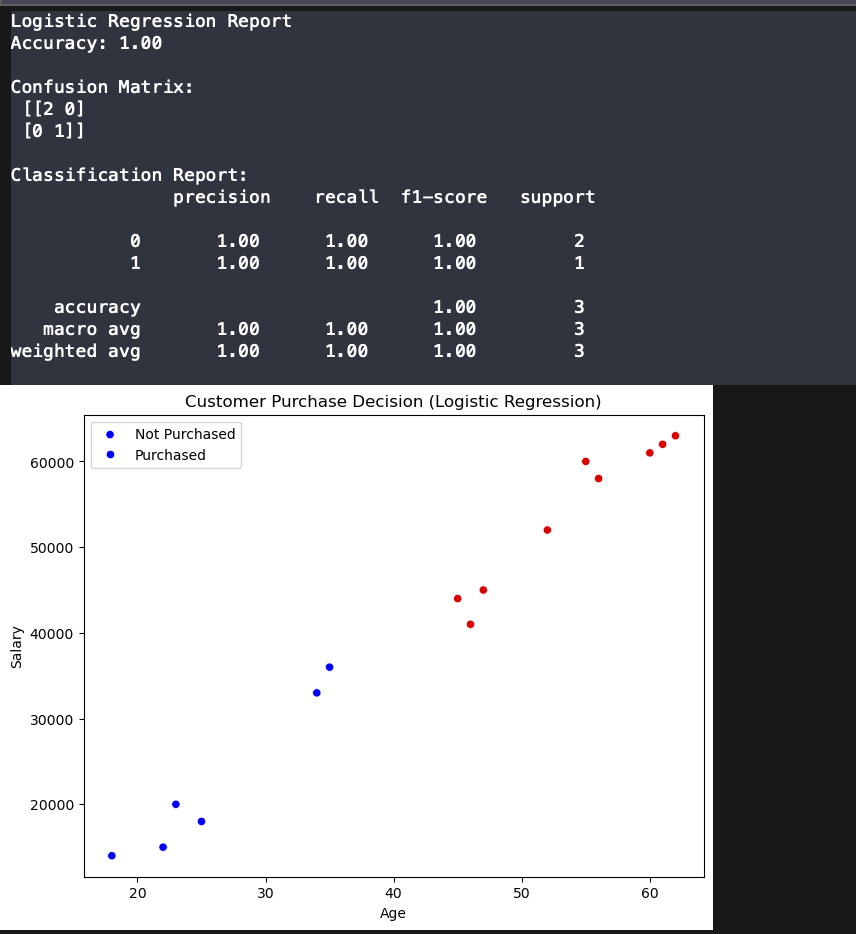
\includegraphics[width=14cm,height=10
cm]{Logistic_Output.png}
    \item \textbf{K-Nearest Neighbors (KNN)}: Classifies as per majority class of k-nearest neighbors.

    \textbf{Example}: Classifying a flower species based on the species of its nearest neighbors.

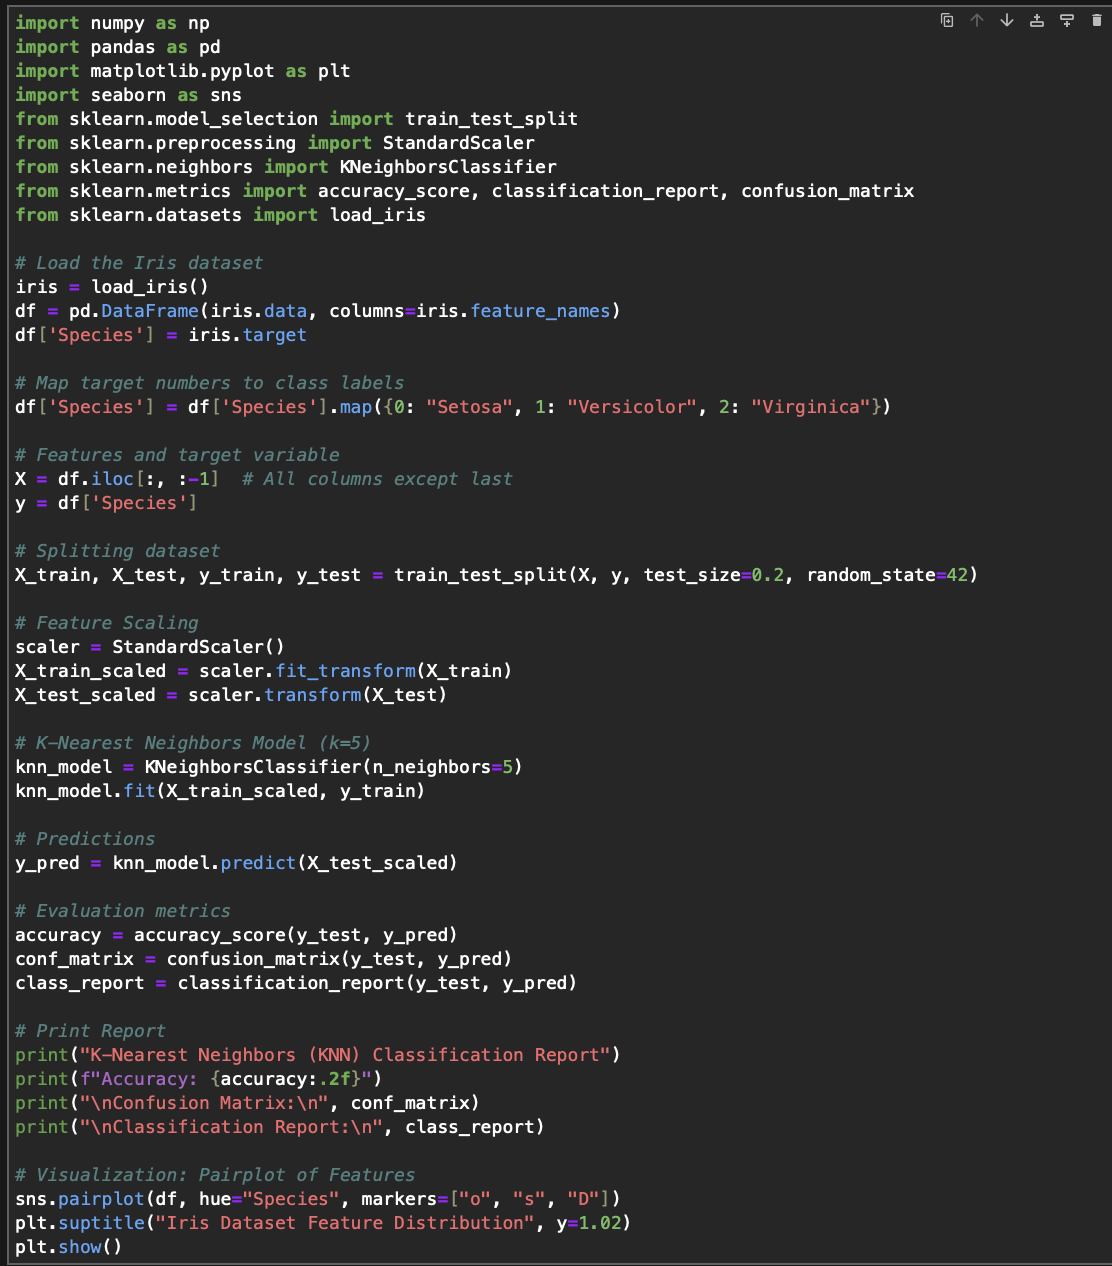
\includegraphics[width=14cm,height=13cm]{KNN.png}

\newpage
\textbf{Output}:

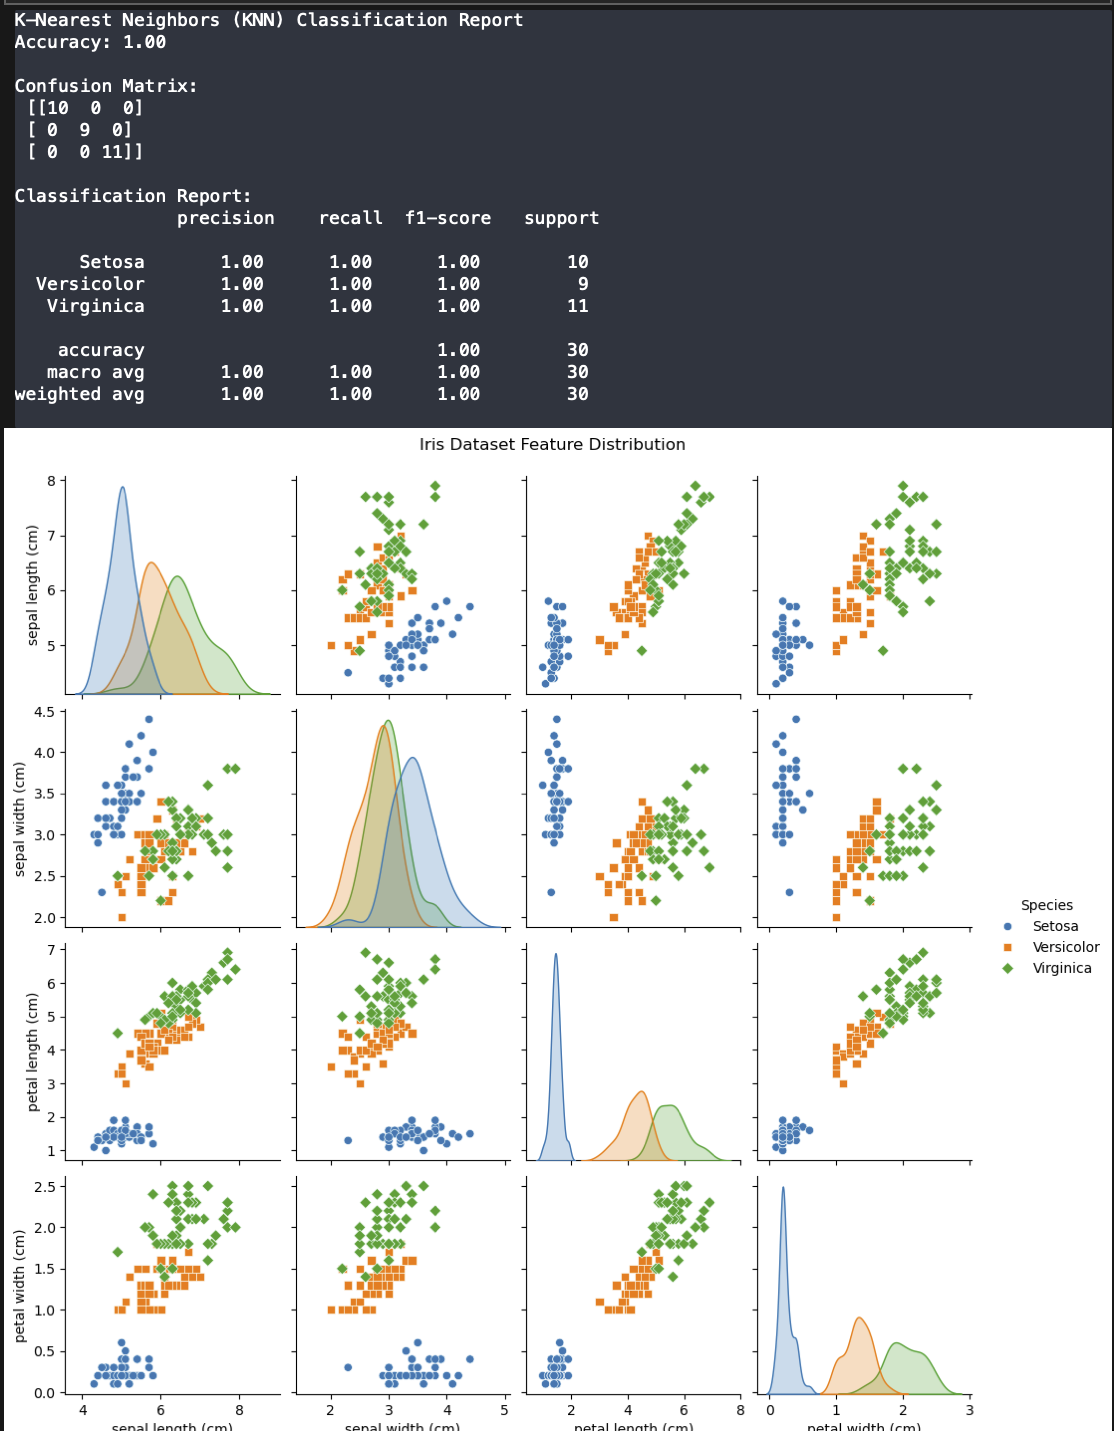
\includegraphics[width=14cm,height=12
cm]{KNN_Output.png}
 \newpage   
    \item \textbf{Decision Tree \& Random Forest}: Hierarchical decision-based tree decision models.

    \textbf{Example of Decision Tree}: Classifying whether a loan applicant is high or low risk based on income and credit score.
    
    \textbf{Example of Random Forest}: Improving loan risk classification by combining multiple decision trees.

    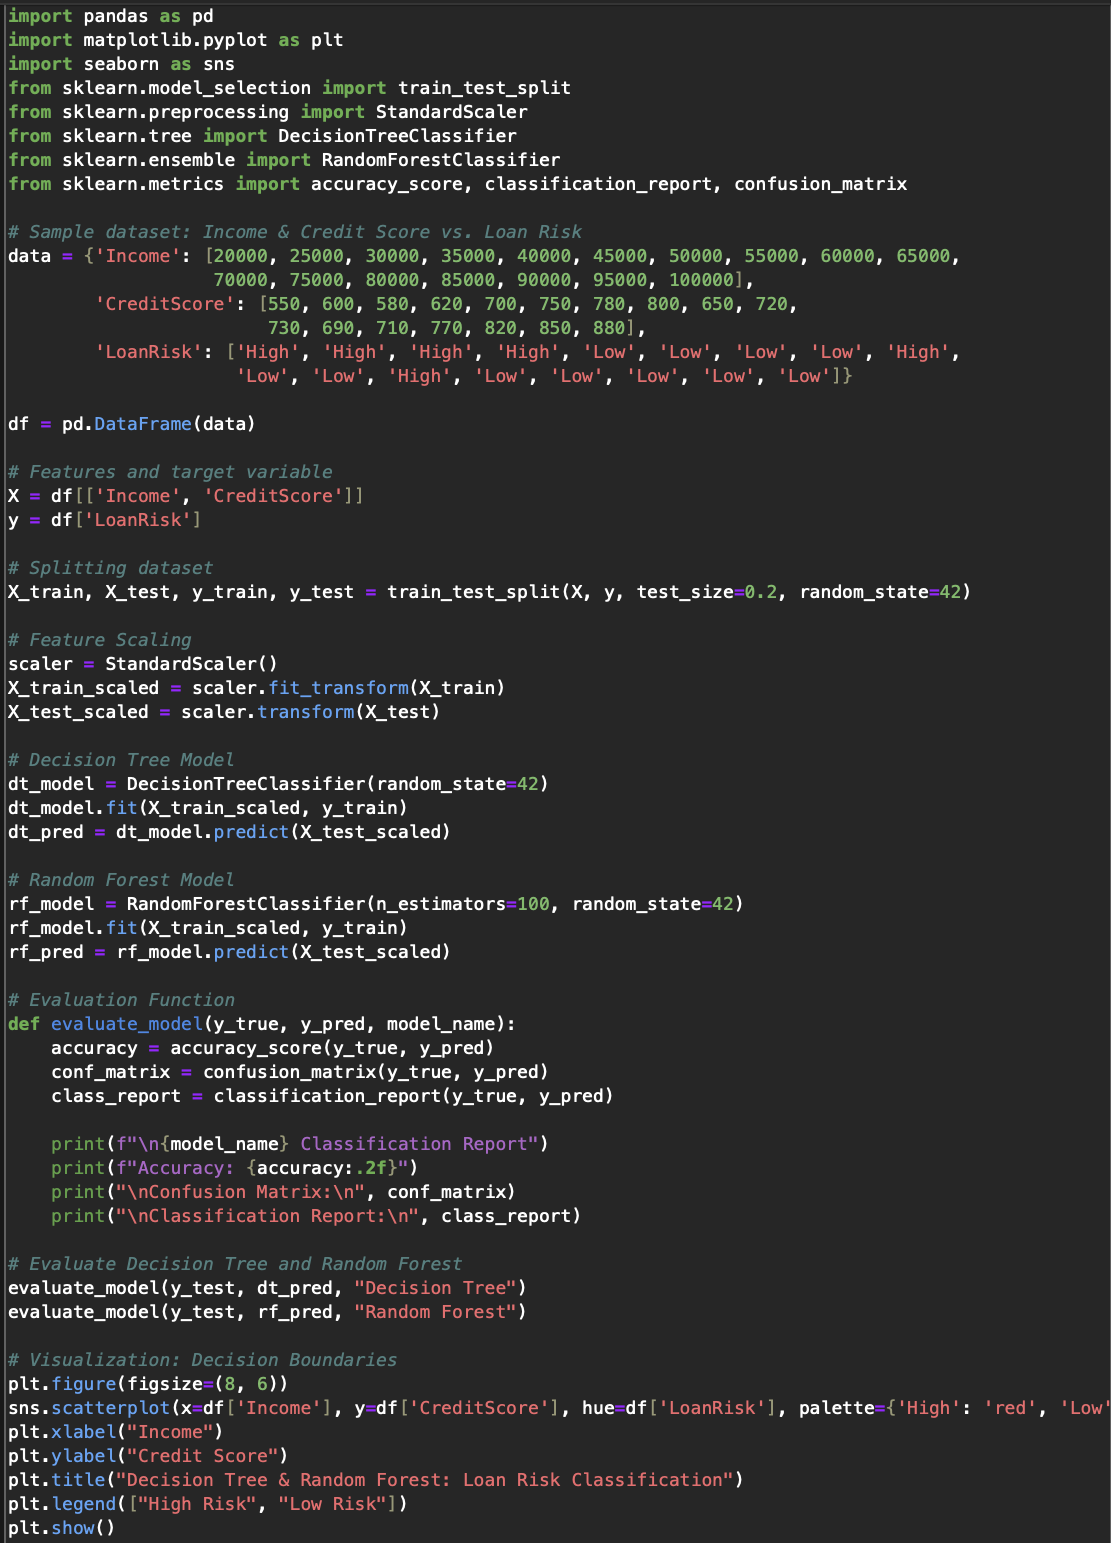
\includegraphics[width=14cm,height=18cm]{Decision Tree.png}

\newpage
\textbf{Output}:

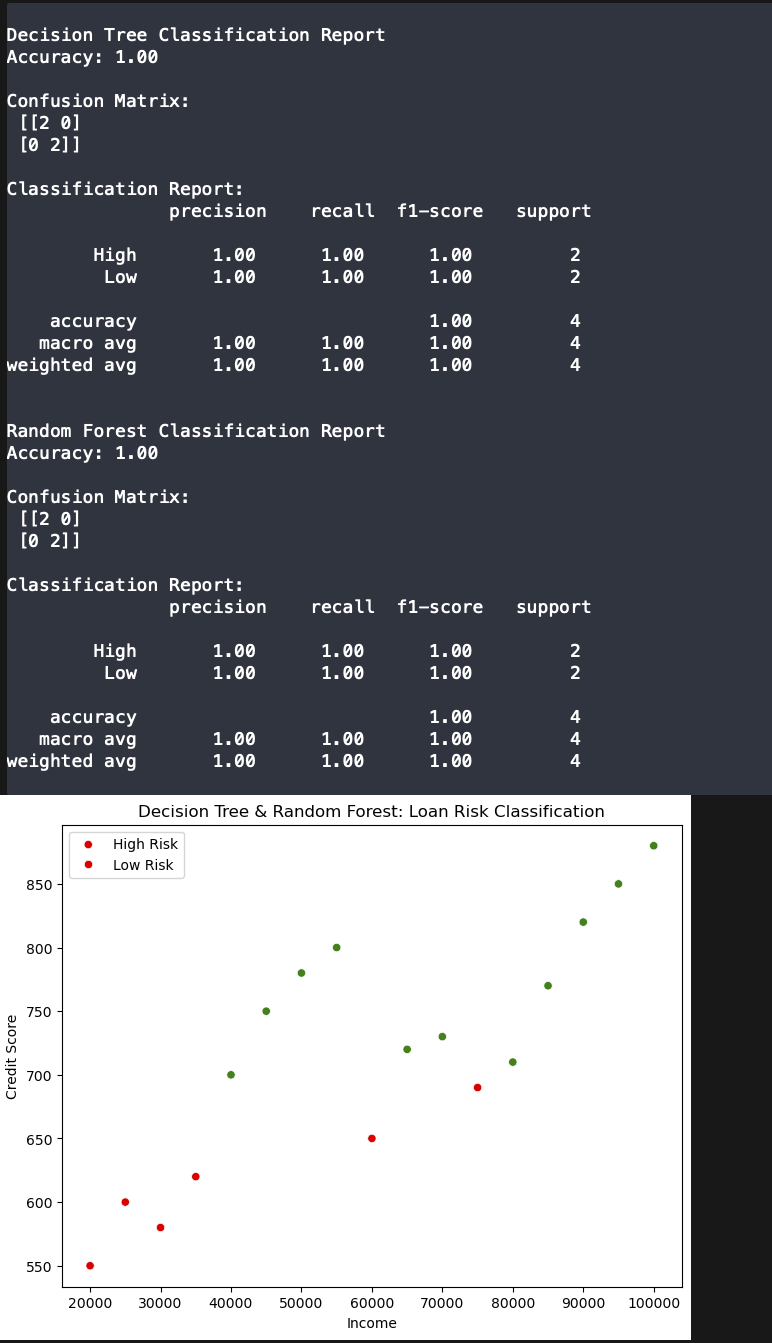
\includegraphics[width=14cm,height=14
cm]{Decision Tree_Output.png}
\newpage
    \item \textbf{Support Vector Machine (SVM)}: Hyperplane-based classification.

    \textbf{Example}: Classifying emails as spam or not spam by finding the optimal decision boundary.

    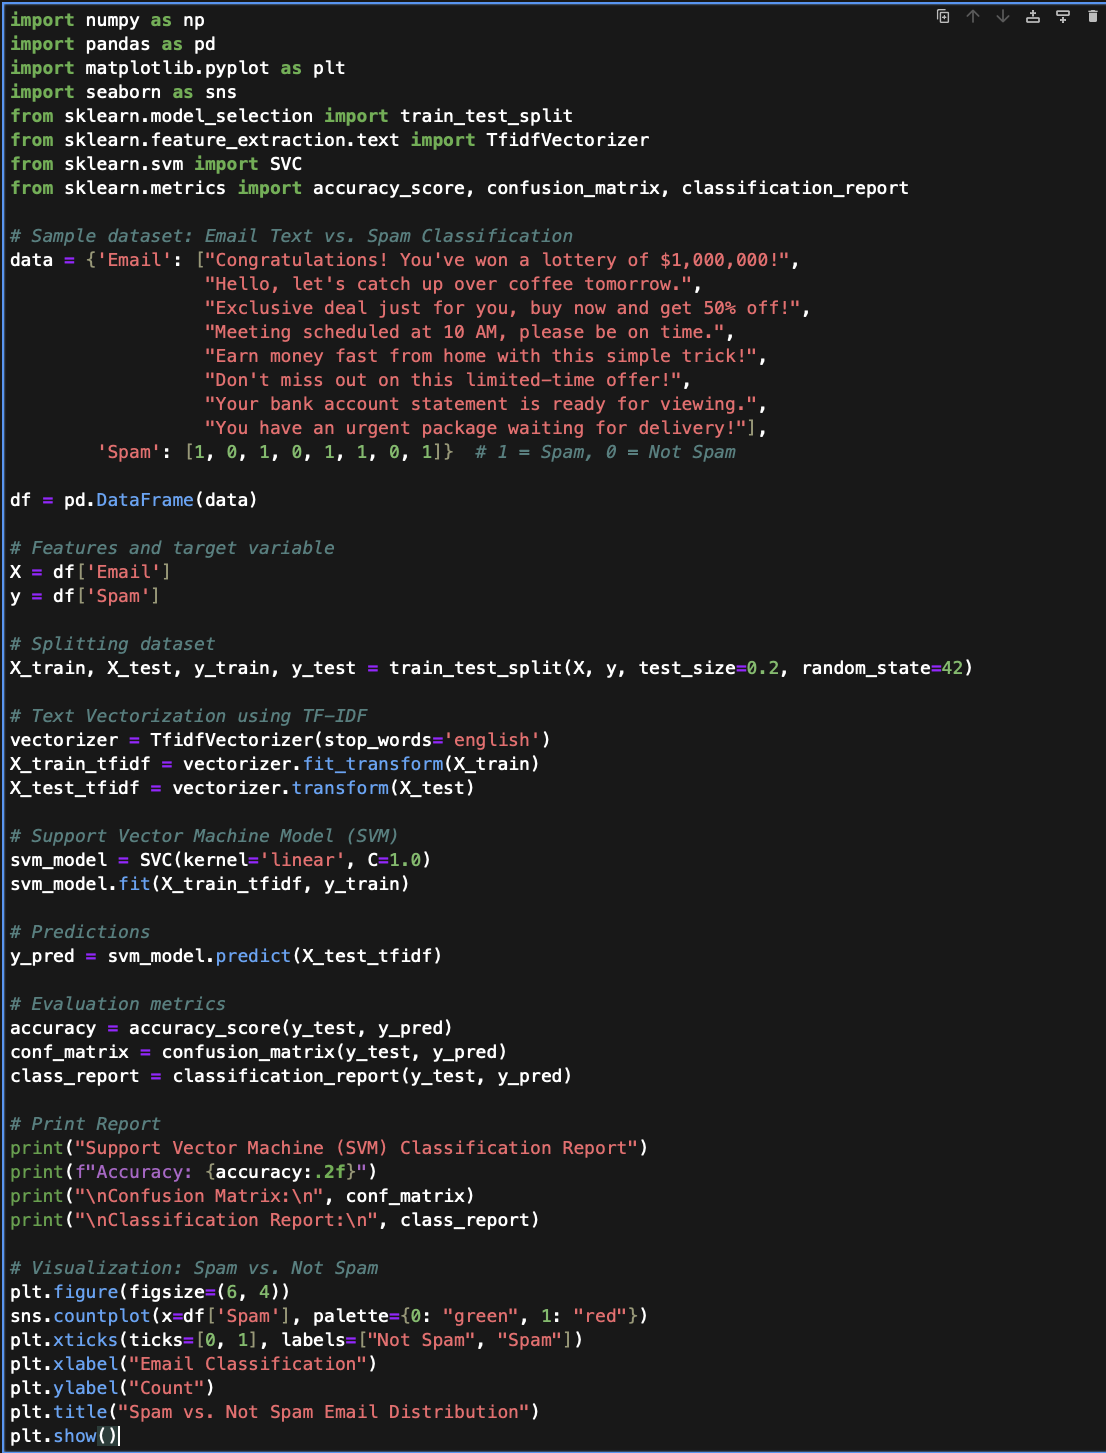
\includegraphics[width=14cm,height=18cm]{SVM.png}

\newpage
\textbf{Output}:

\includegraphics[width=14cm,height=6
cm]{SVM_Output.png}
    \item \textbf{Neural Networks}: Deep networks for complex classification tasks.

    \textbf{Example}: Recognizing handwritten digits from images using multiple layers of neurons.

    \includegraphics[width=14cm,height=16cm]{Neural.png}

\newpage
\textbf{Output}:

\includegraphics[width=14cm,height=12
cm]{Neural_Output.png}
    \end{itemize}
\end{itemize}
\newpage
\subsection{Clustering}
 \begin{itemize}
    \item Clustering is an unsupervised learning method employed to cluster similar data points.
    \item \textbf{Important Methods}:
    \begin{itemize}
    \item \textbf{K-Means Clustering}: Divides data into k clusters based on similarity.

    \textbf{Example}: Grouping customers based on shopping behavior.

    \includegraphics[width=14cm,height=18cm]{K-Means.png}

\newpage
\textbf{Output}:

\includegraphics[width=14cm,height=10
cm]{K-Means_Output.png}
\newpage
    \item \textbf{Hierarchical Clustering}: Constructs a tree of clusters.

    \textbf{Example}: Organizing species into a tree-like structure based on genetic similarity.

    \includegraphics[width=14cm,height=12cm]{Hierarchical.png}


\textbf{Output}:

\includegraphics[width=14cm,height=11
cm]{Hierarchical_Output.png}
    \item \textbf{DBSCAN (Density-Based Clustering)}: Detects clusters based on density.
    
    \textbf{Example}: Identifying clusters of customers based on purchasing patterns while ignoring outliers.

    \includegraphics[width=14cm,height=14cm]{DBSCAN.png}


\textbf{Output}:

\includegraphics[width=14cm,height=8
cm]{DBSCAN_Output.png}
\newpage
    \item \textbf{Gaussian Mixture Models (GMMs)}: Employ probabilistic models to determine cluster membership.

    \textbf{Example}: Segmenting customers into overlapping groups based on purchasing behavior.

    \includegraphics[width=14cm,height=14cm]{Gaussia.png}


\textbf{Output}:

\includegraphics[width=14cm,height=8
cm]{Gaussia_Output.png}
    \end{itemize}
\end{itemize}
\subsection{Model Evaluation}
\begin{itemize}
    \item Model assessment ensures that machine learning models generalize effectively to new, unseen data.
    \item \textbf{Important Methods}:
    \begin{itemize}
    \item \textbf{Regression Metrics}: Mean Squared Error (MSE), R² Score, Mean Absolute Error (MAE).
    \item \textbf{Classification Metrics}: Accuracy, Precision, Recall, F1-score, ROC-AUC.
    \item \textbf{Clustering Metrics}: Silhouette Score, Davies-Bouldin Index, Adjusted Rand Index.
    \end{itemize}
    \item Cross-validation techniques such as k-fold cross-validation and train-test splits aid in model performance evaluation.
\end{itemize}

\includegraphics[width=14cm,height=14cm]{Evaluation.png}


\textbf{Output}:

\includegraphics[width=14cm,height=4
cm]{Evaluation_Output.png}

\subsection{Hyperparameter Tuning}
\begin{itemize}
    \item Hyperparameter tuning enhances the performance of models by selecting the best hyperparameter combination.
    \item \textbf{Important Methods}:
    \begin{itemize}
    \item \textbf{Grid Search}: Attempts the specified set of hyperparameters.

    \includegraphics[width=14cm,height=8cm]{Grid.png}


\textbf{Output}:

\includegraphics[width=14cm,height=1
cm]{Grid_Output.png}
    \item \textbf{Random Search}: Selects hyperparameters randomly from a range.

    \includegraphics[width=14cm,height=6cm]{Random .png}


\textbf{Output}:

\includegraphics[width=14cm,height=2
cm]{Random_Output.png}

\newpage
    \item \textbf{Bayesian Optimization}: Utilizes probabilistic methods to select the best hyperparameters.

    \includegraphics[width=14cm,height=6cm]{Bayesian.png}


\textbf{Output}:

\includegraphics[width=14cm,height=1
cm]{Bayesian_Output.png}
    \item \textbf{Automated Tuning with Optuna \& Hyperopt}: Sophisticated techniques for inexpensive hyperparameter search.

\includegraphics[width=14cm,height=6cm]{Automated.png}


\textbf{Output}:

\includegraphics[width=14cm,height=8.5
cm]{Automated_Output.png}
    \end{itemize}
\end{itemize}

\newpage
\section{ Deep Learning with Python}
Deep learning is a branch of machine learning that deals with training artificial neural networks to identify patterns in data. Python offers strong libraries like TensorFlow and PyTorch for the development of deep learning models. This section introduces important deep learning concepts and methods.
\subsection{Basics of Neural Networks}
\begin{itemize}
    \item Deep Learning and neural networks constitute the majority of this framework, where one is stacked upon another in a sequence of layers of artificial neurons.
    \item \textbf{Key Components}:
    \begin{itemize}
    \item \textbf{Neurons}: Minimum units of information that receive, process, and produce output information.
    \item \textbf{Activation Functions}: Contain non-linearity 
    
    \textbf{Example}: ReLU, Sigmoid, Tanh.
    \item \textbf{Loss Functions}: Compute error between model prediction 
    
    \textbf{Example}: MSE for regression, Cross-Entropy for classification.
    \item \textbf{Optimization Algorithms}: Adjust network weights
    
    \textbf{Example}: Gradient Descent, Adam Optimizer.
    \item \textbf{Backpropagation}: Weights update during gradients for loss reduction.

    \end{itemize}
\end{itemize}

\includegraphics[width=14cm,height=6cm]{Basic.png}


\textbf{Output}:

\includegraphics[width=14cm,height=6
cm]{Basic_Output.png}
\subsection{Introduction to TensorFlow \& PyTorch}
\begin{itemize}
\item TensorFlow and PyTorch are the most popular deep learning frameworks.
\item \textbf{TensorFlow}: Created by Google, has support for computational graphs, TensorFlow Serving for serving, and Keras for a high-level API.

\includegraphics[width=14cm,height=8cm]{TensorFlow.png}


\textbf{Output}:

\includegraphics[width=14cm,height=4
cm]{TensorFlow_Output.png}
\item \textbf{PyTorch}: Created by Facebook, has support for a dynamic computation graph, simple debugging, and is well-liked in research.

\includegraphics[width=14cm,height=9.5cm]{PyTorch.png}


\textbf{Output}:

\includegraphics[width=14cm,height=3
cm]{PyTorch_Output.png}
\end{itemize}
\subsection{Convolutional Neural Networks (CNNs)}
\begin{itemize}
    \item CNNs are deep learning architectures for image processing and computer vision applications.
    \item \textbf{Example}: Identifying objects in images, like detecting cats and dogs in photos.
    \item \textbf{Important Layers}:
    \begin{itemize}
    \item \textbf{Convolutional Layers}: Derive features from images with filters.
    \item \textbf{Pooling Layers}: Downsize dimensionality without losing important features.
    
    \textbf{Example}: Max Pooling
    \item \textbf{Fully Connected Layers}: Flatten and classify derived features.
    \end{itemize}
\end{itemize}

\includegraphics[width=14cm,height=7cm]{CNN.png}


\textbf{Output}:

\includegraphics[width=14cm,height=6
cm]{CNN_Output.png}
\subsection{Recurrent Neural Networks (RNNs)}
\begin{itemize}
    \item RNNs are used for sequential data like time series and natural language processing (NLP).
    \item \textbf{Example}: Predicting the next word in a sentence based on previous words.
    \item \textbf{Variants}:
    \begin{itemize}
    \item \textbf{Vanilla RNN}: It has memory but has trouble with long sequences.
    \item \textbf{Long Short-Term Memory (LSTM)}: Addresses vanishing gradient issues with memory gates.
    \item \textbf{Gated Recurrent Units (GRUs)}: A simpler version of LSTM with comparable effectiveness.
    \end{itemize}
\end{itemize}

\includegraphics[width=14cm,height=7cm]{RNN.png}


\textbf{Output}:

\includegraphics[width=14cm,height=6
cm]{RNN_Output.png}
\subsection{Transfer Learning \& Pretrained Models}
\begin{itemize}
    \item Transfer learning uses the pretrained models over large datasets and fine-tunes them for certain tasks, making training time much less.
    \item \textbf{Example}: Using a pre-trained ImageNet model to classify medical images with fine-tuning.
    \item \textbf{Some Popular Pretrained Models}:
    \begin{itemize}
    \item \textbf{Image Classification}: VGG16, ResNet, EfficientNet.
    \newpage
    \textbf{Example of VGG16}: Classifying cats and dogs in images using a deep CNN with uniform layers.

    \includegraphics[width=14cm,height=7cm]{VGG16.png}


\textbf{Output}:

\includegraphics[width=14cm,height=4
cm]{VGG16_Output.png}

    \textbf{Example of ResNet}: Identifying objects in images with deep residual learning to prevent vanishing gradients.

\includegraphics[width=14cm,height=7cm]{ResNet.png}

\newpage
\textbf{Output}:

\includegraphics[width=14cm,height=6
cm]{ResNet_Output.png}

    \textbf{Example of EfficientNet}: Classifying plant diseases using a highly optimized and scalable CNN model.

    \includegraphics[width=14cm,height=6cm]{EfficientNet.png}

\textbf{Output}:

\includegraphics[width=14cm,height=6
cm]{EfficientNet_Output.png}
\newpage
    \item \textbf{NLP}: BERT, GPT, T5.

    \textbf{Example of BERT}: Understanding the context of a sentence for sentiment analysis.

    \includegraphics[width=14cm,height=4cm]{BERT.png}

\textbf{Output}:

\includegraphics[width=14cm,height=6
cm]{BERT_Output.png}

    \textbf{Example of GPT}: Generating human-like text for chatbots and content creation.

\includegraphics[width=14cm,height=4cm]{GPT.png}

\textbf{Output}:

\includegraphics[width=14cm,height=4
cm]{GPT_Output.png}
\newpage
    \textbf{Example of T5}: Converting questions into answers using a text-to-text approach.

    \includegraphics[width=14cm,height=6cm]{T5.png}

\textbf{Output}:

\includegraphics[width=14cm,height=3
cm]{T5_Output.png}
    \end{itemize}
\end{itemize}
\newpage

\section{Natural Language Processing (NLP)}
Natural Language Processing (NLP) is an AI discipline that allows computers to process, analyze, and create human language. Python offers potent libraries like NLTK, spaCy, and Transformers to perform NLP tasks. This topic discusses some of the major NLP methods and models.
\subsection{Text Preprocessing}
\begin{itemize}
    \item Text preprocessing is the initial stage of NLP, preparing raw text for examination.
    \item \textbf{Example}: Cleaning and tokenizing text before NLP tasks, like removing stopwords and punctuation.
    \item \textbf{Preprocessing Techniques Used}:
    \begin{itemize}
    \item \textbf{Tokenization}: Breaking text into words or sentences.
    
    \textbf{Example}: Splitting a sentence into words or subwords, like "Hello, world!" → ["Hello", ",", "world", "!"].

    \includegraphics[width=14cm,height=4cm]{Tokenization.png}

\textbf{Output}:

\includegraphics[width=14cm,height=2
cm]{Tokenization_Output.png}
    \item \textbf{Stopword removal}: Deleting common words (such as "the," "is") contributing minimal meaning.

    \textbf{Example}: Removing common words like “the,” “is,” and “and” from text to focus on meaningful words.

    \includegraphics[width=14cm,height=4cm]{Stopword.png}

\textbf{Output}:

\includegraphics[width=14cm,height=2
cm]{Stopword_Output.png}
\newpage

     \item \textbf{Stemming \& Lemmatization}: Shrinking words into base forms.

     \textbf{Example of Stemming}: Converting “running” to “run” by trimming suffixes.

\includegraphics[width=14cm,height=2cm]{Stemming.png}

\textbf{Output}:

\includegraphics[width=14cm,height=1
cm]{Stemming_Output.png}

     \textbf{Example of Lemmatization}: Converting “better” to “good” using linguistic rules.

     \includegraphics[width=14cm,height=4cm]{Lemmatization.png}

\textbf{Output}:

\includegraphics[width=14cm,height=1
cm]{Lemmatization_Output.png}
     \item \textbf{Lowercasing}: Lowering everything to lower case.

     \textbf{Example}: Converting “Hello World” to “hello world” for uniform text processing.

\includegraphics[width=14cm,height=2cm]{Lowercasing.png}

\textbf{Output}:

\includegraphics[width=14cm,height=1
cm]{Lowercasing_Output.png}
     \item \textbf{Removing Punctuation \& Special Characters}: Making text ready for consistency.

     \textbf{Example}: Removing Punctuation \& Special Characters.

    \includegraphics[width=14cm,height=2cm]{Punctuation.png}

\textbf{Output}:

\includegraphics[width=14cm,height=1
cm]{Punctuation_Output.png}
    \end{itemize}
\end{itemize}
\newpage
\subsection{TF-IDF \& Word Embeddings}
\begin{itemize}
   \item \textbf{TF-IDF (Term Frequency-Inverse Document Frequency)}: TF-IDF is a quantitative measure that indicates the significance of a word in a document compared to a set of documents.

   \textbf{Example}: Identifying important words in a news article by giving higher scores to rare but meaningful terms like “pandemic” while downweighting common words like “the.”

   \includegraphics[width=14cm,height=6cm]{TF-IDF.png}

\textbf{Output}:

\includegraphics[width=14cm,height=4
cm]{TF-IDF_Output.png}
    \item \textbf{Word Embeddings}: TF-IDF is a quantitative measure that indicates the significance of a word in a document compared to a set of documents.
    \begin{itemize}
    \item \textbf{Word2Vec (Google)}: Learns word relationships.

    \textbf{Example}: Mapping similar words like “king” and “queen” close together in a vector space, capturing semantic relationships.

    \includegraphics[width=14cm,height=8cm]{Word2Vec.png}

\textbf{Output}:

\includegraphics[width=14cm,height=8
cm]{Word2Vec_Output.png}
    \item \textbf{GloVe (Stanford)}: Represents word co-occurrence in corpora.

    \textbf{Example}: Representing words like “coffee” and “café” similarly based on their co-occurrence in large text corpora.

    \includegraphics[width=14cm,height=8cm]{GloVe.png}

\textbf{Output}:

\includegraphics[width=14cm,height=1
cm]{GloVe_Output.png}
\newpage
    \item \textbf{FastText (Facebook)}: Performs well on rare words and subword information.

    \textbf{Example}: Better handling rare words like “unicorn” by breaking them into subword units like “uni” and “corn.”

    \includegraphics[width=14cm,height=8cm]{FastText.png}

\textbf{Output}:

\includegraphics[width=14cm,height=1
cm]{FastText_Output.png}
    \end{itemize}
\end{itemize}
\subsection{Sentiment Analysis \& Named Entity Recognition (NER)}
\begin{itemize}
\item \textbf{Sentiment Analysis}: Sentiment analysis identifies the sentiment (positive, negative, neutral) of a text.

\textbf{Example}: Analyzing customer reviews to determine if the sentiment is positive, negative, or neutral (e.g., “This product is amazing!” → Positive).

\includegraphics[width=14cm,height=8cm]{Sentiment.png}

\textbf{Output}:

\includegraphics[width=14cm,height=1
cm]{Sentiment_Output.png}
\item \textbf{Named Entity Recognition (NER)}: NER detects entities (e.g., names, locations, organizations) in text.

\textbf{Example}: Extracting entities like “Barack Obama” (person), “New York” (location), and “Microsoft” (organization) from the sentence “Barack Obama visited Microsoft headquarters in New York.”

\includegraphics[width=14cm,height=8cm]{NER.png}

\textbf{Output}:

\includegraphics[width=14cm,height=2
cm]{NER_Output.png}
\end{itemize}
\newpage
\subsection{Transformer Models}
\begin{itemize}
\item Transformer models have transformed NLP as they allow deep contextual comprehension.
\item \textbf{Popular Transformer Models}: 
\begin{itemize}
\item \textbf{BERT (Bidirectional Encoder Representations from Transformers)}: Contextual embeddings.

\textbf{Example}: Understanding the meaning of the word “bank” in the context of “river bank” vs. “financial bank” by processing text bidirectionally.

\includegraphics[width=14cm,height=6cm]{BERT.png}

\textbf{Output}:

\includegraphics[width=14cm,height=4
cm]{BERT_Output.png}
\item \textbf{GPT (Generative Pre-trained Transformer)}: Text generation, completion.

\textbf{Example}: Generating coherent and contextually relevant text for applications like chatbots or content creation (e.g., completing a sentence: “The weather is great today, so I decided to…”).

\includegraphics[width=14cm,height=6cm]{GPT2_Output.png}
\newpage
\textbf{Output}:

\includegraphics[width=14cm,height=4
cm]{GPT2.png}
\item \textbf{T5 (Text-to-Text Transfer Transformer)}: Multi-modal text-based learning.

\textbf{Example}: Converting tasks like translation, summarization, and question-answering into a text-to-text framework (e.g., translating “Hello” to “Bonjour”).

\includegraphics[width=14cm,height=6cm]{T52.png}

\textbf{Output}:

\includegraphics[width=14cm,height=4
cm]{T52_Output.png}
\end{itemize}
\end{itemize}
 \newpage
\section{Time Series Analysis}
Time series analysis is concerned with analyzing and predicting data that varies over time. This section introduces the most important techniques for handling time data, detecting trends, seasonality, and generating predictions with statistical and deep learning models.
\subsection{Working with Time-Based Data}
\begin{itemize}
\item Time-based information is recorded sequentially over time at regular intervals.
\item To work efficiently with time series data, time formatting, parsing, and indexing need to be addressed.
\item \textbf{Key Steps}:
\begin{itemize}
\item \textbf{Time Indexing}: Convert timestamps to a pandas DatetimeIndex for easy time-based computation.

\textbf{Example}: Converting a column of timestamps like ["2025-03-01", "2025-03-02"] into a DatetimeIndex in pandas for efficient time-based operations.

\includegraphics[width=14cm,height=6cm]{Resampling.png}

\textbf{Output}:

\includegraphics[width=14cm,height=2.5
cm]{Resampling_Output.png}

\item \textbf{Resampling}: Group data by altering frequencies (i.e., daily to monthly).

\textbf{Example}: Changing daily stock prices to monthly averages using pandas resampling 
(data.resample('M')
.mean()).

\includegraphics[width=14cm,height=6cm]{Resampling.png}

\textbf{Output}:

\includegraphics[width=14cm,height=3cm]{Resampling_Output.png}
\item \textbf{Missing Data}: Treat missing time intervals using interpolation or forward/backward fill.

\textbf{Example}: Filling missing temperature data for specific days by using forward fill (data.fillna(method='ffill')) or interpolation (data.interpolate()).

\includegraphics[width=14cm,height=8cm]{Missing.png}

\textbf{Output}:

\includegraphics[width=14cm,height=10
cm]{Missing_Output.png}
\end{itemize}
\end{itemize}
\subsection{Moving Averages, Seasonality, and Trends}
\begin{itemize}
\item When dealing with time series data, we mostly seek underlying structures such as seasonality and trend.
\item \textbf{Important Methods}:
\begin{itemize}
\item \textbf{Moving Averages}: Removes short-term fluctuations in order to highlight longer-term trends. You can calculate a moving average over a window in order to observe the general trend more easily.

\textbf{Example}: Smoothing out daily stock prices by applying a 7-day moving average to reveal a clearer long-term trend.

\includegraphics[width=14cm,height=8cm]{Moving Averages.png}

\textbf{Output}:

\includegraphics[width=14cm,height=8
cm]{Moving Averages_Output.png}
\newpage
\item \textbf{Simple Moving Average}: Average of a set number of previous observations.

\textbf{Example}: Calculating a 7-day average of website traffic to observe weekly trends and smooth out fluctuations.

\includegraphics[width=14cm,height=8cm]{Simple.png}

\textbf{Output}:

\includegraphics[width=14cm,height=8
cm]{Simple_Output.png}

\newpage
\item \textbf{Exponential Moving Average (EMA)}: Weighted mean where the more recent data are assigned greater weights.

\textbf{Example}: Using a 10-day EMA for stock prices, where more recent days have a higher impact on the average, highlighting the latest market trends.

\includegraphics[width=14cm,height=8cm]{EMA.png}

\textbf{Output}:

\includegraphics[width=14cm,height=8
cm]{EMA_Output.png}
\newpage
\item \textbf{Seasonality}: A regular, typical pattern in the long term. 

\textbf{Example}: Observing that retail sales peak every December due to the holiday season, indicating a seasonal pattern in the data.

\includegraphics[width=14cm,height=8cm]{Seasonality.png}

\textbf{Output}:

\includegraphics[width=14cm,height=8
cm]{Seasonality_Output.png}
\newpage
\item \textbf{Trends}: Trend refers to the direction of the data overall (up or down trend). Trends are employed in making future value forecasts.

\textbf{Example}: Noticing an upward trend in monthly sales over the last few years, suggesting a growth in demand.

\includegraphics[width=14cm,height=8cm]{Trends.png}

\textbf{Output}:

\includegraphics[width=14cm,height=8
cm]{Trends_Output.png}
\end{itemize}
\end{itemize}
\newpage
\subsection{ARIMA, SARIMA, and LSTMs for Forecasting}
\begin{itemize}
\item Time series forecasting uses past observations to forecast future values.
\item \textbf{Most widely used forecasting models}:
\begin{itemize}
\item \textbf{ARIMA (AutoRegressive Integrated Moving Average)}: ARIMA is the most common forecasting model for stationary time series data. ARIMA is an intermix of autoregression (AR), differencing (I), and moving averages (MA).

\textbf{Example}: Predicting next month’s sales based on past sales data, using autoregression to correlate past values, differencing to make the data stationary, and moving averages to smooth out random fluctuations.

\includegraphics[width=14cm,height=16cm]{ARIMA .png}
\newpage
\textbf{Output}:

\includegraphics[width=14cm,height=14
cm]{ARIMA _Output.png}

\includegraphics[width=14cm,height=8
cm]{ARIMA _Output2.png}
\newpage
\item \textbf{AR (AutoRegressive)}: Used the connection between an observation and a set of lagged observations.

\textbf{Example}: Forecasting future stock prices based on a set of previous stock prices (lags), such as using the last 3 days of prices to predict the next day.

\includegraphics[width=14cm,height=18cm]{AR.png}
\newpage
\textbf{Output}:

\includegraphics[width=14cm,height=18
cm]{AR_Output.png}
\newpage
\item \textbf{I (Integrated)}: It makes the time series stationary by calculating the difference between current and lagged observation.

\textbf{Example}: Making a time series stationary by calculating the difference between the current month’s temperature and the previous month’s temperature to remove trends.

\includegraphics[width=14cm,height=18cm]{I.png}
\newpage
\textbf{Output}:

\includegraphics[width=14cm,height=18
cm]{I_Output.png}
\newpage
\item \textbf{MA (Moving Average)}: It indicates the way an observation is connected to a residual error in a moving average model.

\textbf{Example}: Using the past 5 days of errors (the difference between predicted and actual values) to predict future stock prices.

\includegraphics[width=14cm,height=20cm]{MA .png}
\newpage
\textbf{Output}:

\includegraphics[width=14cm,height=6cm]{MA _Output.png}
\item \textbf{SARIMA (Seasonal ARIMA)}: It's a form of ARIMA that takes seasonality into consideration. It's used when your data is seasonal.

\textbf{Example}: Predicting future energy consumption by considering yearly seasonal patterns (e.g., higher usage in winter) and using SARIMA for seasonal adjustments.

\includegraphics[width=14cm,height=16cm]{SARIMA.png}
\newpage
\textbf{Output}:

\includegraphics[width=14cm,height=18
cm]{SARIMA_Output.png}
\newpage
\item \textbf{LSTM (Long Short-Term Memory)}: Deep learning model that excels at predicting whether there are long-term dependencies in time series data. LSTMs are a type of Recurrent Neural Networks (RNN) and excel at predicting future patterns from a sequence of data.

\textbf{Example}: Using LSTM models to forecast traffic patterns by learning long-term dependencies in historical data, such as predicting next week’s traffic based on patterns observed over several months.

\includegraphics[width=14cm,height=18cm]{LSTM.png}

\includegraphics[width=14cm,height=4cm]{LSTM2.png}

\textbf{Output}:

\includegraphics[width=14cm,height=18
cm]{LSTM_Output.png}

\end{itemize}
\end{itemize}

\newpage
\section{Big Data \& Distributed Computing}
In the era of big data, efficiently processing and managing large amounts of data is an important challenge. Distributed computing libraries and frameworks serve to address this challenge by allowing parallel processing and scaling to deal with large datasets. This section presents some influential tools and techniques for working with big data using Python.
\subsection{Using Dask and Vaex for Large Datasets}
\begin{itemize}
\item If working with large data that cannot be stored in memory, one can utilize libraries like Vaex and Dask.
\item These support parallel computation in large-scale data processing.
\item \textbf{Dask}:
\begin{itemize}
\item An adaptive parallelism library that is compatible with current libraries such as Pandas and NumPy.
\item Dask divides large tasks into small ones and spreads them across many machines or cores, so it's perfect for working with large data.
\item \textbf{Dask DataFrame}: Similar to Pandas DataFrame but can process data sets that are too big to hold in memory by dividing them into smaller, more manageable chunks.
\item \textbf{Dask Arrays}: Like NumPy arrays but distributed across machines or multiple cores.
\item\textbf{Example}: Using Dask to process a large dataset of customer transactions that won’t fit into memory by breaking the data into smaller chunks and processing them across multiple cores or machines, just like working with a Pandas DataFrame.

\includegraphics[width=14cm,height=4cm]{Dask.png}

\textbf{Output}:

\includegraphics[width=14cm,height=2
cm]{Dask_Output.png}
\end{itemize}

\newpage
\item \textbf{Vaex}:
\begin{itemize}
\item A memory-frugal and rapid library for the manipulation of massive tabular datasets (billions of rows).
\item It relies on lazy evaluation, i.e., it does not load data into memory until that's needed, enabling you to process larger-than-memory datasets seamlessly.
\item\textbf{Example}: Analyzing a billion-row dataset of user activity logs without loading all data into memory at once, using Vaex’s lazy evaluation to only load the data needed for computation.

\includegraphics[width=14cm,height=6cm]{Vaex.png}

\textbf{Output}:

\includegraphics[width=14cm,height=2
cm]{Vaex_Output.png}
\end{itemize}
\end{itemize}
\subsection{Introduction to Apache Spark (PySpark)}
\begin{itemize}
\item Apache Spark is an open-source distributed computing system for quick big data processing.
\item It offers APIs for data processing on various nodes of a cluster.
\item \textbf{PySpark}: Python API for Spark, enabling Python developers to take advantage of the power of Spark for processing large data.

\textbf{Example}: Using PySpark to process and analyze a massive dataset of user clicks across multiple nodes of a cluster, speeding up computation compared to traditional methods.

\includegraphics[width=14cm,height=8cm]{PySpark.png}

\textbf{Output}:

\includegraphics[width=14cm,height=3
cm]{PySpark_Output.png}
\item \textbf{Spark SQL}: Spark module that enables querying of data with SQL-like syntax. Useful for people who are familiar with SQL but wish to work with big data.

\textbf{Example}: Querying a large dataset of sales transactions with SQL-like syntax (SELECT * FROM sales WHERE amount $>$ 100), but leveraging Spark’s distributed power for faster execution on big data.

\includegraphics[width=14cm,height=8cm]{Spark.png}

\textbf{Output}:

\includegraphics[width=14cm,height=4
cm]{Spark_Output.png}
\newpage
\item \textbf{Resilient Distributed Datasets (RDDs)}: The underlying data structure for Spark, where data can be distributed and processed in parallel. 

\textbf{Example}: Storing and processing distributed data across a cluster, like splitting a large log file into chunks and processing them in parallel to find error patterns.

\includegraphics[width=14cm,height=8cm]{RDD.png}

\textbf{Output}:

\includegraphics[width=14cm,height=2
cm]{RDD_Output.png}
\item Spark finds extensive usage for big data operations such as ETL (Extract, Transform, Load), machine learning, and real-time processing.

\end{itemize}
\newpage
\subsection{Parallel Processing and Scalability}
\begin{itemize}
\item Parallel processing refers to the method of breaking down work into small sub-tasks that are executed in parallel between multiple systems or processors.
\item Parallel processing plays a crucial role in big data since it allows for faster computation through efficient utilization of available resources.
\item \textbf{Multithreading}: Running multiple threads in a single process to perform tasks concurrently.

\textbf{Example}: Running multiple threads within a single Python process to handle different parts of a data cleaning pipeline concurrently, improving efficiency on tasks like file reading or string processing.

\includegraphics[width=14cm,height=8cm]{Multithreading.png}

\textbf{Output}:

\includegraphics[width=14cm,height=3
cm]{Multithreading_Output.png}
\newpage
\item \textbf{Multiprocessing}: Spawning multiple processes to run on separate CPUs or cores, which is ideal for CPU-bound tasks.

 \textbf{Example}: Using Python’s multiprocessing library to process large CSV files in parallel, dividing the workload across multiple CPU cores to speed up data analysis.

 \includegraphics[width=14cm,height=6cm]{Multiprocessing.png}

\textbf{Output}:

\includegraphics[width=14cm,height=1
cm]{Multiprocessing_Output.png}
\item \textbf{Distributed Computing}: Execution of tasks on several machines (distributed system) through tools such as Dask, Spark, or Hadoop. 

\textbf{Example}: Leveraging Apache Spark to split a large dataset of customer transactions across several machines and process them in parallel, significantly reducing processing time compared to a single machine.

\includegraphics[width=14cm,height=8cm]{Distributed.png}

\textbf{Output}:

\includegraphics[width=14cm,height=3
cm]{Distributed_Output.png}
\item \textbf{Scalability}:
\begin{itemize}
\item Means the capacity of a system to cope with increasing data effectively.
\item Big data software and platforms such as Dask and Spark are built to be highly scalable, as they can process much bigger datasets than the memory or storage capacity of an individual machine.
\item \textbf{Example}: Using Spark or Dask to process a growing dataset, ensuring the system can handle increased data volume by distributing the workload across more resources (machines, CPUs).

\includegraphics[width=14cm,height=6cm]{Scalability.png}

\textbf{Output}:

\includegraphics[width=14cm,height=2
cm]{Scalability_Output.png}
\end{itemize}
\end{itemize}
\newpage
\section{Data Science Best Practices \& Deployment}
In data science, it's essential not only to develop successful models but also ones that are understandable, deployable, and scalable. This topic addresses best practice for model explainability, deployment, version management, and ethical use when employing AI and machine learning models.
\subsection{Model Interpretability}
\begin{itemize}
\item Model interpretability involves the capability to comprehend and describe how a model comes to a decision.
\item As machine learning models, particularly sophisticated ones such as deep learning networks, grow stronger, they can become "black boxes," such that it is challenging to describe their predictions.
\item \textbf{There are a number of techniques and methods of model interpretability improvement}: 
\begin{itemize}
\item \textbf{Feature Importance}: Identifying which features (variables) are most important for the model’s predictions.

\textbf{Example}: Using a Random Forest model to identify which features, such as age or income, most influence the prediction of whether a customer will buy a product.

\includegraphics[width=14cm,height=6cm]{Feature.png}

\textbf{Output}:

\includegraphics[width=14cm,height=2
cm]{Feature_Output.png}
\newpage
\item \textbf{LIME (Local Interpretable Model-Agnostic Explanations)}: An approach to explaining a single prediction by locally fitting the model with a simpler, interpretable model.

\textbf{Example}: Using LIME to explain why a machine learning model predicted a specific loan rejection, by creating a simpler model that approximates the complex model’s behavior near that specific data point.

\includegraphics[width=14cm,height=6cm]{LIME .png}

\textbf{Output}:

\includegraphics[width=14cm,height=4
cm]{LIME _Output.png}
\item \textbf{SHAP (SHapley Additive exPlanations)}: A game theory-inspired method to explain any machine learning model prediction by distributing the prediction value across features.

\textbf{Example}: Using SHAP to explain a model’s prediction on a housing price, showing how each feature (location, size, age) contributed to the predicted price by distributing the prediction value across those features.

\includegraphics[width=14cm,height=6cm]{SHAP.png}
\newpage
\textbf{Output}:

\includegraphics[width=14cm,height=6
cm]{SHAP_Output.png}
\end{itemize}
\end{itemize}
\subsection{Model Deployment}
\begin{itemize}
\item Deploying a machine learning model is deploying it to production wherein the model is utilized by end-users or systems.
\item Deployment then comes into play to make the model scalable and useable.
\item \textbf{Model Serving}: 
\begin{itemize}
\item It is hosting the model in a format which is being served via an API so that other apps or people can even make predictions.
\item The model is distributed via APIs of frameworks like Flask or FastAPI.
\item \textbf{Example}: Hosting a fraud detection model via a FastAPI service so that other applications can make real-time predictions on transaction data by calling the API.

\includegraphics[width=14cm,height=6
cm]{Model.png}
\end{itemize}
\item \textbf{Model Monitoring}:
\begin{itemize}
\item Once implemented, monitoring the performance of the model constantly in real time is necessary so that it would always be functioning at its peak.
\item Methods such as A/B testing and detection of drift are used to keep a lookout for problems such as model degradation with time.
\item \textbf{Example}: Using A/B testing to compare a newly deployed recommendation model with the previous one to see if it provides better results or detecting drift by monitoring performance over time to catch any degradation in accuracy.

\includegraphics[width=14cm,height=4
cm]{Monitoring.png}
\end{itemize}
\item \textbf{Containerization}:
\begin{itemize}
\item Software such as Docker enables you to bundle your model and its dependencies into a deployable container across various environments.
\item \textbf{Example}: Using Docker to package a sentiment analysis model along with its required libraries and dependencies, ensuring that the model can be deployed consistently across different environments (development, staging, production).

\includegraphics[width=14cm,height=4
cm]{Containerization.png}
\end{itemize}
\end{itemize}
\subsection{Version Control for ML Models}
\begin{itemize}
\item Version control is an essential aspect of machine learning to maintain model, dataset, and code versions in sync over time.
\item This facilitates reproducibility and model evolution to be handled more easily.

\item \textbf{Git}:
\begin{itemize}
\item Although Git is widely used for code versioning, it may also be utilized for model versioning.
\item For big files such as datasets and models, however, you might rather have tools like Git LFS (Large File Storage) or DVC (Data Version Control) at your disposal.
\item \textbf{Example}: Using Git to manage changes to your machine learning codebase and workflows while employing Git LFS for large files like pre-trained models or datasets.

\textbf{Setup}:

\includegraphics[width=14cm,height=4
cm]{Git.png}
\end{itemize}
\item \textbf{DVC}:
\begin{itemize}
\item DVC is a version control system that is model and machine learning data-specific.
\item It is used to version and track models, datasets, and experiments without keeping large files in Git itself.
\item \textbf{Example}: Using DVC to track different versions of your model and datasets during experimentation, so you can easily reproduce results and ensure that the model and its training data are properly versioned.

\textbf{Setup}:

\includegraphics[width=14cm,height=4
cm]{DVC.png}
\end{itemize}
\end{itemize}
\subsection{ Ethical Considerations and Bias in AI}
\begin{itemize}
\item As the usage of machine learning and artificial intelligence algorithms grew, it is crucial to manage the AI bias and ethical issues in such a manner that it becomes fair and not become a catastrophic entity.
\item \textbf{AI Bias}:
\begin{itemize}
\item AI bias in training data could create models that make biased or discriminatory choices. 
\item One must strictly prepare and examine the data for the possibility of bias opportunities.
\item \textbf{Example}: If a facial recognition system is trained on predominantly white faces, it may perform poorly or inaccurately on individuals from other racial backgrounds, leading to biased results.

\end{itemize}
\item \textbf{Fairness}:
\begin{itemize}
\item AI models must be made equitable to everyone and not prejudicial to a section of the population. 
\item Methods such as Fairness Constraints and Bias Mitigation can be utilized to minimize unfair outcomes.
\item \textbf{Example}: Ensuring a hiring algorithm does not discriminate against candidates based on gender or ethnicity by applying fairness constraints that remove biases from training data or model predictions.


\end{itemize}
\item \textbf{Accountability and Transparency}:
\begin{itemize}
\item AI systems must be transparent to ensure stakeholders are aware of how decisions are being made. 
\item Models must be maintained as interpretable and explainable, which is a central aspect of this.
\item \textbf{Example}: Providing clear explanations to stakeholders on how a loan approval model makes decisions, ensuring that the process is interpretable and justifiable to avoid discrimination and maintain trust.
\end{itemize}
\item \textbf{Privacy}:
\begin{itemize}
\item Artificial intelligence systems must maintain the privacy and security of users, particularly in processing sensitive personal data.
\item \textbf{Example}: Implementing data anonymization techniques in healthcare AI systems to protect patient identities while ensuring that sensitive medical data used for training models remains secure and private.
\end{itemize}
\item \textbf{Example Tool}: 
\begin{itemize}
\item \textbf{IBM AI Fairness 360 (AIF360)}: Detecting Bias in a Dataset.
\item \textbf{Fairlearn}: Mitigating Bias in a Classifier.
\item \textbf{SHAP}: Explaining Model Decisions.
\item \textbf{Google What-If Tool}: Interactive Bias Analysis.
\end{itemize}
\end{itemize}
\newpage
\section{Conclusion}
\begin{itemize}
\item \textbf{Data Science with Python}: Python is really the sweetheart language in science data because of how beautiful it is, the great culture of libraries, and because bringing intelligent support bases together is simply so strong.
\item \textbf{Data Acquisition \& Processing}: Interleaving data processing with file handling, web scraping, APIs, and data cleansing gives good quality data for analysis.
\item \textbf{Exploratory Data Analysis (EDA)}: EDA, which stands for Exploratory Data Analysis, which is a whole bunch of cool stuff like cool stats summaries, cool data visualization, and cool methods of dimension reduction that are all great at showing insights and patterns.
\item \textbf{Python Machine Learning}: Unsupervised and supervised learning activities like regression, classification, clustering, model selection, and hyperparameter tuning improve prediction power.
\item \textbf{Deep Learning \& Neural Networks}: Advanced deep learning systems that are really sophisticated like using CNNs for stuff like vision, RNNs for things with time—like stock quotes or speech records—plus transformers that excel at language processing deliver super high performance in high class models.
\item \textbf{Natural Language Processing (NLP)}: Word embeddings, TF-IDF, processing of text, sentiment analysis and transformer models all work really well together for working with textual information. They all work very nicely and complement each other really well. Each one does different things but they are used together to get maximal effectiveness. It's like having a team where each member plays a different role but together they are great.
\item \textbf{Time Series Analysis}: Seasonality detection, moving averages, and time-series forecasting models like ARIMA, SARIMA, and LSTMs can be applied on time-based data.
\item \textbf{Big Data \& Distributed Computing}: Dask, Vaex and Apache Spark (which uses Python Spark called pyspark) are super good at big data processing and doing computing work on super big sets of data at the same time.
\item \textbf{Model Deployment \& Versioning}: Model deployment with Flask, FastAPI, and cloud computing and versioning with Git, DVC, and MLflow provide reproducibility and reliability.
\item \textbf{Ethical Issues \& Model Explainability}: AI fairness management, bias detection, and interpretability through methods like SHAP and LIME provide ethical AI.
\item \textbf{Final Thoughts}:Python remains king for data science because pragmatic pros want to analyze, process and implement data solutions that scale while playing nice with ethics  so that they can make powerful AI adoption happen.
\end{itemize}

\end{document}